\pdfminorversion=4 % avoid compatibility problems with embedded PNGs in Adobe Acrobat
%% \documentclass[handout,t]{beamer} % HANDOUT
%% \documentclass[handout,notes=show,t]{beamer} % NOTES
\documentclass[t]{beamer} % SLIDES
\usepackage{etex}

\usetheme{StefanFAU}                % page themes: StefanPlain, StefanFAU, StefanOsna
%% \usepackage{beamer-font-lucida}  % commercial Lucida Math font package (recommended)
%% \usepackage{beamer-font-charter} % commercial Charter Match font package
%% \usepackage{beamer-font-arev}    % use Arev fonts from TexLive (combine with document option "smaller")
\usepackage{beamer-tools-stefan}    % standard packages, definitions and macros

%%%% uncomment the following macro libraries as needed
%% %%
%% support macros for graphics with the PGF packages
%%

%% \mmpaper[black]{0}{0}{8}{5}, \xypaper{0}{0}{8}{5}
%%   draw fine grid in pgf picture so that objects can easily be positioned
%%   \mmpaper draws cm/mm blocks, while \xypaper is based on (x,y) coordinates
\newcommand{\mmpaper}[5][black!40!white]{
  \begin{pgfscope}
    \color{#1}
    \pgfsetlinewidth{.2mm}
    \pgfgrid[step={\pgfpoint{1cm}{1cm}}]{\pgfpoint{#2cm}{#3cm}}{\pgfpoint{#4cm}{#5cm}}
    \pgfsetlinewidth{.1mm}
    \pgfgrid[step={\pgfpoint{1mm}{1mm}}]{\pgfpoint{#2cm}{#3cm}}{\pgfpoint{#4cm}{#5cm}}
  \end{pgfscope}
}
\newcommand{\xypaper}[5][black!40!white]{
  \begin{pgfscope}
    \color{#1}
    \pgfsetlinewidth{.2mm}
    \pgfgrid[step={\pgfxy(1,1)}]{\pgfxy(#2,#3)}{\pgfxy(#4,#5)}
    \pgfsetlinewidth{.1mm}
    \pgfgrid[step={\pgfxy(.1,.1)}]{\pgfxy(#2,#3)}{\pgfxy(#4,#5)}
  \end{pgfscope}
}

%%% Local Variables: 
%%% mode: latex
%%% TeX-master: ""
%%% End: 
   % basic PGF utility functions
%%
%% some macros for typesetting text
%%

%% \OPEN ... \CLOSE; \OPEN[np] ... \CLOSE[np]
%% bold large brackets for labelled bracketing notation
\newcommand<>{\OPEN}[1][]{\only#2{$\boldsymbol{\bigl[}\text{}_{\text{\raisebox{-2pt}{\textsc{#1}}}}$}}
\newcommand<>{\CLOSE}[1][]{\only#2{$\text{}_{\text{\raisebox{-2pt}{\textsc{#1}}}}\boldsymbol{\bigr]}$}}

%% \textgap ("_" representing missing letter)
\newcommand{\textgap}{\mbox{\hspace{.4pt}\texttt{\bfseries\secondary{\textunderscore}}\hspace{.4pt}}}

%% \textstar, \textast (math \star and \ast symbols in text mode, with some extra spacing)
\newcommand{\textstar}{$\mspace{.8mu}\star\mspace{.8mu}$}
\newcommand{\textast}{$\ast$}

%% $\p{\ctext{abc}}$ (cited text in mathematical equations, e.g. n-gram probabilities)
\newcommand{\ctext}[1]{\text{\textcite{#1}}}

%% $\p{\btext{abc}}$ (normal black text even in coloured math environment)
\newcommand{\btext}[1]{\text{\foreground{#1}}} 

%% text subscripts and superscripts (can be used in math and text mode)
\newcommand{\tsup}[1]{\ensuremath{^{\text{#1}}}}
\newcommand{\tsub}[1]{\ensuremath{_{\text{#1}}}}

%%% Local Variables: 
%%% mode: latex
%%% TeX-master: ""
%%% End: 
  % some macros for typesetting text
%%
%% some useful macros: mathematical notation etc.
%%

%% abbreviations for logic symbols
\renewcommand{\implies}{\Rightarrow}
\newcommand{\equivalent}{\Leftrightarrow}

%% abbreviations for common number spaces
\newcommand{\setN}[1][]{\mathbb{N}_{#1}} % allows \setN and \setN[0]
\newcommand{\setZ}{\mathbb{Z}}
\newcommand{\setQ}{\mathbb{Q}}
\newcommand{\setR}{\mathbb{R}}

%% sets and (sub-)sets defined by condition
\newcommand{\set}[1]{\{#1\}}
\newcommand{\setdef}[2]{\set{#1\,|\,#2}}
\newcommand{\bigset}[1]{\bigl\{#1\bigr\}}
\newcommand{\bigsetdef}[2]{\bigset{#1\bigm|#2}}
\newcommand{\setscale}[1]{\left\{#1\right\}}
\newcommand{\setdefscale}[2]{\setscale{#1\left|\,#2\right.}}

%% absolute value and norm
\newcommand{\abs}[1]{\lvert #1\rvert}
\newcommand{\bigabs}[1]{\bigl\lvert #1\bigr\rvert}
\newcommand{\absscale}[1]{\left\lvert #1\right\rvert}
\newcommand{\norm}[2][]{\lVert #2\rVert_{#1}}
\newcommand{\bignorm}[2][]{\bigl\lVert #2\bigr\rVert_{#1}}
\newcommand{\normscale}[2][]{\left\lVert #2\right\rVert_{#1}}

%% complement set (with optional index)
\newcommand{\compl}[1][]{\mathcal{C}^{#1}}

%% power set: \powerset{\Sigma^*}
\newcommand{\powerset}[1]{\mathcal{P}(#1)}

%% uparrow: a \ua b = direct dominance in ordered tree
\newcommand{\ua}{\uparrow}

%% left-right arrow: this $\lra$ that
\newcommand{\lra}{\leftrightarrow}

%% expanded engineering notation: 4.2\x\e+5
\newcommand{\e}[2]{10^{\ifthenelse{\equal{#1}{+}}{}{#1}#2}}
\newcommand{\x}{\cdot}

%% arg max & min: \argmax_{x\in C}, \argmin_{x\in C}
\newcommand{\argmax}{\mathop{\text{arg~max}}}
\newcommand{\argmin}{\mathop{\text{arg~min}}}

%% infinitesimal elements: \dx, \dy = \dX{y}, \dz
\newcommand{\dX}[1]{\,\mathit{d{#1}}}
\newcommand{\dx}{\dX{x}}
\newcommand{\dy}{\dX{y}}
\newcommand{\dz}{\dX{z}}

%%% Local Variables: 
%%% mode: latex
%%% TeX-master: ""
%%% End: 
  % basic mathematical notation
%%
%% some useful macros: statistical notation
%%

%% \p{X=k};  \pC{X=k}{Y=l};  \bigp{X_i = k};   \pscale{\frac{Z}{S^2}};
%% probability P(X=k) and conditional probability P(X=k|Y=l), also with larger or scaled parentheses
%% \p[\theta]{X=k};  \pC[\text{interpolated}]{X=k}{Y=l};  ...
%% with optional subscripts (for model probability, null probability, etc.)
\newcommand{\p}[2][]{\mathop{\mathrm{Pr}_{#1}}(#2)}
\newcommand{\pscale}[2][]{\mathop{\mathrm{Pr}_{#1}}\!\left(#2\right)}
\newcommand{\bigp}[2][]{\mathop{\mathrm{Pr}_{#1}}\bigl(#2\bigr)}
\newcommand{\pC}[3][]{\p[#1]{#2\,|\,#3}} 
\newcommand{\pCscale}[3][]{\pscale[#1]{#2\left|\,#3\right.\!}} 
\newcommand{\bigpC}[3][]{\bigp[#1]{#2\!\bigm|\!#3}} 

%% \Exp{X};  \Var{X};  \Exp[0]{X};  \Var[0]{X};  
%% \bigExp{X}; \bigVar{X}; \Expscale{X};  \Varscale{X};
%% expectation E[X] and variance V[X], expectation and variance under null hypothesis, 
%% and variants with largeer or scaled brackets
\newcommand{\Exp}[2][]{\mathrm{E}_{#1}[#2]}
\newcommand{\Var}[2][]{\mathop{\mathrm{Var}}_{#1}[#2]}
\newcommand{\bigExp}[2][]{\mathrm{E}_{#1}\!\bigl[#2\bigr]}
\newcommand{\bigVar}[2][]{\mathop{\mathrm{Var}}_{#1}\bigl[#2\bigr]}
\newcommand{\Expscale}[2][]{\mathrm{E}_{#1}\left[#2\right]}
\newcommand{\Varscale}[2][]{\mathop{\mathrm{Var}}_{#1}\left[#2\right]}

%% \pihat = \hat{\pi}
%% sampling estimate for population probability \pi (may need fine-tuning)
\newcommand{\pihat}{\hat{\pi}}

%% \Entropy{X}, \Entropy{p}, \KL{p}{q}, \MI{X}{Y}
%% \bigEntropy{}, \Entropyscale{}, \bigKL{}{}, \KLscale{}{}, \bigMI{}{}, \MIscale{}{}
%% entropy, KL distance, conditional entropy and mutual information (with scaled variants)
\newcommand{\Entropy}[1]{H[{#1}]}
\newcommand{\bigEntropy}[1]{H\bigl[{#1}\bigr]}
\newcommand{\Entropyscale}[1]{H\left[{#1}\right]}
\newcommand{\KL}[2]{D({#1}\|{#2})}
\newcommand{\bigKL}[2]{D\bigl({#1}\bigm\|{#2}\bigr)}
\newcommand{\KLscale}[2]{D\left({#1}\left\|{#2}\right.\right)}
\newcommand{\MI}[2]{I[{#1};{#2}]}
\newcommand{\bigMI}[2]{I\bigl[{#1};{#2}\bigr]}
\newcommand{\MIscale}[2]{I\left[{#1};{#2}\right]}

%% \corr (correlation) and \cov (covariance) as mathop's
\newcommand{\corr}{\mathop{\mathrm{corr}}}
\newcommand{\cov}{\mathop{\mathrm{cov}}
}
%%% Local Variables: 
%%% mode: latex
%%% TeX-master: ""
%%% End: 
  % notation for probability theory and statistics
%%
%% convenience macros for linear algebra (vectors and matrices)
%%

%% \Vector[i]{x} ... vector variable with optional _superscript_ index in parentheses
%% \Vector[']{x} ... special case: ' superscript not enclosed in parentheses
%% \vx, \vy, \vz ... abbreviations for common vector names
\newcommand{\Vector}[2][]{\vec{#2}\ifthenelse{\equal{#1}{}}{}{^{(#1)}}}
\newcommand{\vx}[1][]{\Vector[#1]{x}}
\newcommand{\vy}[1][]{\Vector[#1]{y}}
\newcommand{\vz}[1][]{\Vector[#1]{z}}
\newcommand{\vu}[1][]{\Vector[#1]{u}}
\newcommand{\vv}[1][]{\Vector[#1]{v}}
\newcommand{\vw}[1][]{\Vector[#1]{w}}
\newcommand{\va}[1][]{\Vector[#1]{a}} % vectors of coefficients
\newcommand{\vb}[1][]{\Vector[#1]{b}} % for basis
\newcommand{\ve}[1][]{\Vector[#1]{e}} % for standard basis of R^n
\newcommand{\vn}[1][]{\Vector[#1]{n}} % normal vector
\newcommand{\vnull}[1][]{\Vector[#1]{0}} % neutral element

%% \Span{\vb[1],\ldots,\vb[k]} ... span of set of vectors
%% \Rank{...} ... rank of set of vectors or matrix
%% \Det{...}, \det A ... determinant of a set of vectors / a matrix A
%% \Image{f}, \Kernel{f} ... image and kernel of a linear map
\newcommand{\Span}[1]{\mathop{\text{sp}}\left(#1\right)}
\newcommand{\Rank}[1]{\mathop{\text{rank}}\left(#1\right)}
\newcommand{\Det}[1]{\mathop{\text{Det}}\left(#1\right)}
%% \det is already defined in the standard library
\newcommand{\Image}[1]{\mathop{\text{Im}}\left(#1\right)}
\newcommand{\Kernel}[1]{\mathop{\text{Ker}}\left(#1\right)}

%% \dist[2]{\vx}{\vy} ... distance between two vectors (p-metric)
\newcommand{\dist}[3][]{d_{#1}\left(#2, #3\right)}
\newcommand{\bigdist}[3][]{d_{#1}\bigl(#2, #3\bigr)}

%% \sprod{\vu}{\vv} ... scalar product
\newcommand{\sprod}[2]{\left\langle #1, #2 \right\rangle}
\newcommand{\bigsprod}[2]{\bigl\langle #1, #2 \bigr\rangle}


%%% Local Variables: 
%%% mode: latex
%%% TeX-master: ""
%%% End: 
% convenience macros for vectors and matrices
%% %%
%% grid-like layout of strings etc in PGF picture
%%

\usepackage{calc}

%% configure grid layout and style:
%%   \setGridOrigin{<x>}{<y>} ... origin of grid
%%   \setGridX{3cm}           ... unit on x-axis (columns)
%%   \setGridY{1cm}           ... unit on y-axis (rows)
%%   \setGridAlignment{left}{base} ... alignment of elements in grid
%%   \renewcommand{\gridStyle}[1]{\small\secondary{#1}}
\newlength{\gridOriginX}  \setlength{\gridOriginX}{0cm}
\newlength{\gridOriginY}  \setlength{\gridOriginY}{0cm}
\newlength{\gridXunit}    \setlength{\gridXunit}{3cm}
\newlength{\gridYunit}    \setlength{\gridYunit}{1em}
\newcommand{\setGridOrigin}[2]{%
  \setlength{\gridOriginX}{#1}%
  \setlength{\gridOriginY}{#2}%
}
\newcommand{\setGridX}[1]{\setlength{\gridXunit}{#1}}
\newcommand{\setGridY}[1]{\setlength{\gridYunit}{#1}}
\newcommand{\gridAlignH}{left}
\newcommand{\gridAlignV}{base}
\newcommand{\setGridAlignment}[2]{%
  \renewcommand{\gridAlignH}{#1}%
  \renewcommand{\gridAlignV}{#2}%
}
\newcommand{\gridStyle}[1]{\secondary{\small{}#1}}

%% these are temporary registers for internal use
\newlength{\gridTemp}
\newlength{\gridTempX}
\newlength{\gridTempY}

%% internal: \gridXYcell{<col>}{<row>} -> \gridTempX, \gridTempY
\newcommand{\gridXYcell}[2]{%
  \setlength{\gridTempX}{\gridXunit * \real{#1} + \gridOriginX}%
  \setlength{\gridTempY}{\gridYunit * \real{#2} + \gridOriginY}%
}

%% print text (\pgfbox) in specified cell (Col, Row)
%%   \gridText<overlay>{Col}{Row}{Text}
\newcommand<>{\gridText}[3]{%
  \only#4{%
    \gridXYcell{#1}{#2}%
    \pgfputat{\pgfpoint{\gridTempX}{\gridTempY}}{%
      \pgfbox[\gridAlignH,\gridAlignV]{\gridStyle{#3}}}}%
}


%%% Local Variables: 
%%% mode: latex
%%% TeX-master: ""
%%% End: 
  % grid-like layout of text and graphics in PGF picture
%% %%
%% macros for typesetting parse trees with PGF
%%

\usepackage{calc}

%% configure tree dimensions:
%%   \setlength{\treeHstep}{5mm}, \setlength{\treeVstep}{5mm}
%%   \setTreeHeight{6} -> 6 non-terminal layers above terminal string (default: 8)
%%   \setTreeRelative{3.5} -> slots are specified relative to this position (default: 0)
%%   \setTreeBoxW{Text}, \setTreeBoxH{Text}, \setTreeBoxWH{Text} 
%%      -> set amount of space reserved for tree node (to accommodate Text in current font)
%%
\newlength{\treeHstep}
\setlength{\treeHstep}{10mm}
\newlength{\treeVstep}
\setlength{\treeVstep}{10mm}
\newlength{\treeBoxH}
\newlength{\treeBoxD}
\newlength{\treeBoxW}
%% internal lengths and commands
\newlength{\treeBoxTotalH}
\newlength{\treeBoxBaseDY}
\newcommand{\calculateTreeBox}{%
  \setlength{\treeBoxTotalH}{\treeBoxH + \treeBoxD}%
  \setlength{\treeBoxBaseDY}{\treeBoxD - \treeBoxTotalH / 2}%
}
\newcommand{\setTreeBoxW}[1]{\settowidth{\treeBoxW}{#1}}
\newcommand{\setTreeBoxH}[1]{%
  \settoheight{\treeBoxH}{#1}%
  \settodepth{\treeBoxD}{#1}%
  \calculateTreeBox{}}
\newcommand{\setTreeBoxWH}[1]{\setTreeBoxW{#1}\setTreeBoxH{#1}}
\setTreeBoxW{XX}                % default: W = two wide letters
\setTreeBoxH{Tg}                % default: H = full height + depth
\newcounter{TreeHeight}
\setcounter{TreeHeight}{8}
\newcommand{\setTreeHeight}[1]{\setcounter{TreeHeight}{#1}}
%% internal lengths and commands
\newlength{\treeRelativeX}
\setlength{\treeRelativeX}{0mm}
\newcommand{\setTreeRelative}[1]{\setlength{\treeRelativeX}{\treeHstep * \real{#1}}}

%% these are temporary registers for internal use
\newlength{\treeTemp}
\newlength{\treeTempX}
\newlength{\treeTempY}
\newcounter{TreeTemp}

%% internal: \treeYforLayer{<layer>} -> \treeTempY = y-position
\newcommand{\treeYforLayer}[1]{%
  \setlength{\treeTempY}{\treeVstep * \real{\theTreeHeight} - \treeVstep * \real{#1}}%
}

%% internal: \treeXforSlot{<slot>} -> \treeTempX = x-position
\newcommand{\treeXforSlot}[1]{%
  \setlength{\treeTempX}{\treeRelativeX + \treeHstep * \real{#1}}%
}

%% internal: insert strut for full text line height (to improve text alignment)
\newcommand{\treeStrut}{%
  \settoheight{\treeTemp}{X}\rule{0mm}{\treeTemp}%
}

%% put (non-terminal) tree node in slot <Slot> on layer <Layer>, 
%% labelled with <Text> and assigned the node label <Lab>; 
%% layers count from 0 = root layer at the top of the tree
%%   \treeNode<overlay>{Lab}{Layer}{Slot}{Text}
%%   \treeNodePT<overlay>{Lab}{Slot}{Text} ... on pre-terminal layer
\newcommand<>{\treeNode}[4]{%
  \treeYforLayer{#2}\treeXforSlot{#3}%
  \pgfnoderect{#1}[virtual]{\pgfpoint{\treeTempX}{\treeTempY}}{\pgfpoint{\treeBoxW}{\treeBoxTotalH}}%
  \addtolength{\treeTempY}{\treeBoxBaseDY}%
  \only#5{\pgfputat{\pgfpoint{\treeTempX}{\treeTempY}}{\pgfbox[center,base]{#4}}}%
}
\newcommand<>{\treeNodePT}[3]{%
  \setcounter{TreeTemp}{\theTreeHeight - 1}%
  \treeNode#4{#1}{\theTreeTemp}{#2}{#3}%
}

%% put (terminal) leaf node in slot <Slot> on lexical layer>, 
%% labelled with <Text> and assigned the node label <Lab>
%%   \treeLeaf<overlay>{Lab}{Slot}{Text}
\newcommand<>{\treeLeaf}[3]{%
  \treeNode#4{#1}{\theTreeHeight}{#2}{#3}%
}

%% connect tree nodes with straight (unlabelled) edge
%%   \treeEdge{Lab1}{Lab2}
\newcommand<>{\treeEdge}[2]{%
  \begin{pgfscope}
    \pgfclearstartarrow
    \pgfclearendarrow
    \pgfsetlinewidth{1pt}
    \pgfnodeconnline#3{#1}{#2}
  \end{pgfscope}
}

%% connect tree nodes with curved (unlabelled) edge; leaves upper node
%% Lab1 at Angle relative to vertical, enters lower node Lab2 vertically
%%   \treeEdgeCurve{Lab1}{Angle}{Lab2}
\newcommand<>{\treeEdgeCurve}[3]{%
  \begin{pgfscope}
    \pgfclearstartarrow%
    \pgfclearendarrow%
    \pgfsetlinewidth{1pt}%
    \setcounter{TreeTemp}{#2 - 90}%
    \pgfnodeconncurve#4{#1}{#3}{\theTreeTemp}{90}{\treeVstep}{\treeVstep}
  \end{pgfscope}
}

%% attach note to given node (in right bottom corner)
%%   \treeNote<overlay>[right]{Lab}{Text}
\newcommand<>{\treeNote}[3][left]{%
  \only#4{%
    \pgfputat{\pgfnodeborder{#2}{-60}{-2pt}}{%
      \pgfbox[#1,top]{\setlength{\fboxsep}{1pt}\colorbox{white}{%
          \scriptsize\secondary{\treeStrut{}#3}}}}}%
}

%% represent subtree (root=Root, boundary=Left..Right) as triangle
%%   \treeTriangle<overlay>{Root}{Left}{Right}
\newcommand<>{\treeTriangle}[3]{%
  \begin{pgfscope}
    \only#4{%
      \pgfclearstartarrow%
      \pgfclearendarrow%
      \pgfsetlinewidth{1pt}%
      \pgfmoveto{\pgfnodeborder{#1}{-90}{2pt}}%
      \pgflineto{\pgfnodeborder{#2}{135}{2pt}}%
      \pgflineto{\pgfnodeborder{#3}{45}{2pt}}%
      \pgfclosestroke%
    }
  \end{pgfscope}
}



%%% Local Variables: 
%%% mode: latex
%%% TeX-master: ""
%%% End: 
  % typesetting parse trees with PGF
%% %%
%% macros for demonstrating chart parsers with PGF
%%

\usepackage{calc,ifthen}

%% configure chart dimensions:
%%   \setlength{\chartXunit}{5mm}, \setlength{\chartYunit}{5mm}
%%   \setChartWidth{8}
\newlength{\chartXunit}
\setlength{\chartXunit}{10mm}
\newlength{\chartYunit}
\setlength{\chartYunit}{5mm}
\newcounter{ChartWidth}
\setcounter{ChartWidth}{8}
\newcommand{\setChartWidth}[1]{%
  \setcounter{ChartWidth}{#1}}

%% these are temporary registers for internal use
\newlength{\chartTemp}
\newlength{\chartTempH}
\newlength{\chartTempW}
\newlength{\chartTempX}
\newlength{\chartTempY}

%% internal: \chartXcoord{<x>} -> \chartTempX
\newcommand{\chartXcoord}[1]{%
  \setlength{\chartTempX}{\chartXunit * \real{#1}}%
}

%% internal: \chartYcoord{<y>} -> \chartTempY
\newcommand{\chartYcoord}[1]{%
  \setlength{\chartTempY}{\chartYunit * \real{#1}}%
}

%% internal: \chartXYcoord{<x>}{<y>} -> \chartTempX, \chartTempY
\newcommand{\chartXYcoord}[2]{%
  \chartXcoord{#1}\chartYcoord{#2}%
}

%% internal: insert strut for full text line height (to improve text alignment)
\newcommand{\chartStrut}{%
  \settoheight{\chartTemp}{X}\rule{0mm}{\chartTemp}%
}
 
%% put terminal symbol <Text> in given <Slot> (x-coordinate) with optional label
%%   \chartTerminal<overlay>[Lab]{Slot}{Text}
\newcommand<>{\chartTerminal}[3][chartNULL]{%
  \only#4{%
    \chartXYcoord{#2}{0}
    \settowidth{\chartTempW}{#3}
    \pgfputat{\pgfpoint{\chartTempX}{\chartTempY}}{\pgfbox[center,base]{\chartStrut{}#3}}%
    \addtolength{\chartTempY}{.4em}%
    \pgfnoderect{#1}[virtual]{\pgfpoint{\chartTempX}{\chartTempY}}{%
      \pgfpoint{\chartXunit / 2}{1em}}%
  }
}

%% draw arrow across span of substring at height <Y> and label with <Tag>
%%   \chartSpan[Lab]{Y}{X1}{X2}{Tag}
\newcommand<>{\chartSpan}[5][chartNULL]{%
  \only#6{%
    \chartXYcoord{#3}{#2}%
    \setlength{\chartTemp}{\chartTempX}%
    \chartXcoord{#4}%
    \addtolength{\chartTemp}{\chartXunit * \real{-.35}}%
    \addtolength{\chartTempX}{\chartXunit * \real{.35}}%
    \begin{pgfscope}
      \pgfclearstartarrow{}\pgfsetendarrow{\pgfarrowtriangle{3pt}}%
      \pgfsetlinewidth{1pt}%
      \color{counterpoint}%
      \pgfline{\pgfpoint{\chartTemp}{\chartTempY}}{\pgfpoint{\chartTempX}{\chartTempY}}%
    \end{pgfscope}
    \setlength{\chartTempH}{\chartTempY + \chartYunit * \real{0.4}}%
    \setlength{\chartTempW}{\chartTempX - \chartTemp}%
    \setlength{\chartTempX}{(\chartTemp + \chartTempX) / 2}%
    \pgfnoderect{#1}[virtual]{\pgfpoint{\chartTempX}{\chartTempH}}{\pgfpoint{\chartTempW}{\chartYunit * \real{0.8}}}%
    \addtolength{\chartTempY}{2pt}%
    \pgfputat{\pgfpoint{\chartTempX}{\chartTempY}}{%
      \pgfbox[center,base]{\scriptsize\color{secondary}#5}}%
  }%  
}

%% CFG production for use as span label (LHS in bold)
%%   \charProd{LHS}{RHS}
\newcommand{\chartProd}[2]{%
  \textbf{#1} $\to$ {#2}%
}

%% draw dashed line across entire chart at height <Y>, optional with <Text> on LHS
%%   \chartRule{Y}, \chartRule[Text]{Y}
\newcommand<>{\chartRule}[2][]{%
  \only#3{%
    \begin{pgfscope}
      \chartXYcoord{0}{#2}%
      \setlength{\chartTemp}{\chartTempX}%
      \chartXcoord{\theChartWidth}%
      \addtolength{\chartTemp}{\chartXunit * \real{-.5}}%
      \addtolength{\chartTempX}{\chartXunit * \real{-.5}}%
      \addtolength{\chartTempY}{\chartYunit * \real{.4}}%
      \pgfclearstartarrow{}\pgfclearendarrow{}%
      \pgfsetlinewidth{1pt}%
      \pgfsetdash{{2mm}{2mm}}{1mm}%
      \pgfline{\pgfpoint{\chartTemp}{\chartTempY}}{\pgfpoint{\chartTempX}{\chartTempY}}%
      \addtolength{\chartTemp}{-4pt}%
      \pgfputat{\pgfpoint{\chartTemp}{\chartTempY}}{\pgfbox[right,base]{\small #1}}%
    \end{pgfscope}
  }%  
}

%% draw edge of parse tree into chart (nodes must have been labelled);
%% uses current color (change with \color{...} before drawing edges)
%%   \chartEdge<overlay>{Lab1}{Lab2}
\newcommand<>{\chartEdge}[2]{%
  \begin{pgfscope}
    \pgfclearstartarrow%
    \pgfclearendarrow%
    \pgfsetlinewidth{1.5pt}%
    \pgfnodesetsepstart{2pt}%
    \pgfnodeconnline#3{#1}{#2}%
  \end{pgfscope}
}

%%% Local Variables: 
%%% mode: latex
%%% TeX-master: ""
%%% End: 
 % demonstrating chart parsers with PGF
%% %%
%% some useful macros for formal languages
%%

%% empty word \eps (length \abs{w} defined in math.tex)
\newcommand{\eps}{\epsilon}

%% roman (or sans-serif) letters used as symbols in examples
\newcommand{\z}[1]{\textsf{#1}}

%% language denoted by a given grammar or regular expression
\newcommand{\lang}[2][]{\mathcal{L}_{#1}\bigl[#2\bigr]}

%% language generated by a Turing machine 
\newcommand{\generate}[2][]{\mathcal{G}_{#1}\bigl[#2\bigr]}

%% regular expressions: \reg{expr}, \R(, \R), \R*, ..., \len{\reg{expr}}
\newcommand{\R}[1]{\texttt{#1}}
\newcommand{\reg}[1]{\underline{#1}}
\newcommand{\regeps}{\reg{\eps}}
%\newcommand{\len}[1]{\ell\left(#1\right)} %% do we still need that command?

%% class \langReg[\Sigma] of all regular languages, and set \langR[\Sigma] of all regular expressions
\newcommand{\langReg}[1][\Sigma]{\operatorname{Reg}(#1)}
\newcommand{\langR}[1][\Sigma]{R(#1)}


%%
%% Endliche Automaten
%%


%% Regeln f�r die formale Beschreibung (im Formelmodus zu verwenden):
%%   \Xearule{<lab1>}{<lab2>}{<label>}
%% [<lab1>, <lab2> sind Zustandslabel und werden im Formelmodus gesetzt]
%% [<label> bezeichnet das Eingabezeichen und wird AUCH im FORMELMODUS gesetzt]
%%   \earule{<n1>}{<n2>}{<label>}
%% [<label> bezeichnet das Label einer Bewegung und wird im Textmodus gesetzt]
\newcommand{\earule}[3]{q_{#1} \overset{\text{#3}}{\longrightarrow} q_{#2}}
\newcommand{\Xearule}[3]{#1 \overset{#3}{\longrightarrow} #2}



%%
%% Kontextfreie Grammatiken
%%

%% Ableitungsschritte und Ableitung
%%   \drv[<grammar>]
%%   \Drv[<grammar>]
\newcommand{\drv}[1][]{\implies_{#1}}
\newcommand{\Drv}[1][]{\implies_{#1}^*}

%% class \langKF[\Sigma] of all context-free languages
\newcommand{\langKF}[1][\Sigma]{\operatorname{KF}(#1)}

%% Regeln f"ur die formale Beschreibung von Kellerautomaten (im Formelmodus):
%%   \Xpdarule{<state1>}{<V>}{<label>}{<state2>}{<stack>}
%% [�bergang von Zustand <state1> mit oberem Kellersymbol <V> in
%%  Zustand <state2>, wobei <stack> auf dem Keller abgelegt wird;
%%  dabei wird das Zeichen <label> verarbeitet]
\newcommand{\Xpdarule}[5]{(#1,#2) \overset{#3}{\longrightarrow} (#4,#5)}

%% A \to \alpha \oder \beta ... Disjunktionsstrich mit zus�tzlichem Abstand
\newcommand{\oder}{\,|\,}



%%% Local Variables: 
%%% mode: latex
%%% TeX-master: ""
%%% End: 
    % some notation for formal language theory

%%%
%%% local configuration adjustments
%%%

%%% You can change pre-defined colours here, override built-in macros from the
%%% style definition and standard library, as well as define macros needed by
%%% all local documents.

%%% e.g. adjust counterpoint (dark green) for data projectors where greens are
%%% far too bright, as well as green component of light colour and pure green
%%% (of course, it's a better solution to adjust the gamma settings of your monitor)
%%
%% \definecolor{counterpoint}{rgb}{.1, .3, 0}
%% \definecolor{light}{rgb}{.45, .3, .55}
%% \definecolor{puregreen}{rgb}{0, .35, 0}

%% parenthesized superscript (time step / event token)
\newcommand{\psup}[1]{\ensuremath{^{(#1)}}}
\newcommand{\psupt}{\psup{t}}

\usepackage{tikz}
\usetikzlibrary{positioning}
\usetikzlibrary{arrows.meta}
\usepackage{pgfplots}
 % local adjustments to configuration and macros

%%%%%%%%%%%%%%%%%%%%%%%%%%%%%%%%%%%%%%%%%%%%%%%%%%%%%%%%%%%%%%%%%%%%%%
%% Titlepage

%\title[NDL: From R-W to ML in NLP]{\textbf{Naïve Discriminative Learning:}\\
%  From Rescorla-Wagner to Machine Learning in Natural Language Processing}
\title[NDL: From R-W to ML in NLP]{Naïve Discriminative Learning}
\subtitle{From Rescorla-Wagner to Machine Learning in Natural Language Processing}
\author{Stefan Evert}
\institute[]{%
  Friedrich-Alexander-Universität Erlangen-Nürnberg, Germany\\
  {\secondary{\url{stefan.evert@fau.de}}}
}
\date[Osnabrück, 21.06.2017]{Osnabrück, 21 June 2017}


\begin{document}

%% \showLogo  % uncomment to show logo on title page in StefanPlain style
\frame{\titlepage}
\hideLogo

%%%%%%%%%%%%%%%%%%%%%%%%%%%%%%%%%%%%%%%%%%%%%%%%%%%%%%%%%%%%%%%%%%%%%%
%% Outline

\section*{Outline}
\frame{ 
  \frametitle{Outline}
  \tableofcontents
}
\AtBeginSubsection[]
{
  \begin{frame}
    \frametitle{Outline}
    \tableofcontents[current,currentsubsection]
  \end{frame}
}

%%%%%%%%%%%%%%%%%%%%%%%%%%%%%%%%%%%%%%%%%%%%%%%%%%%%%%%%%%%%%%%%%%%%%%
%% 1 Introduction
\section{Introduction}

%%%%%%%%%%%%%%%%%%%%%%%%%%%%%%%%%%%%%%%%%%%%%%%%%%%%%%%%%%%%%%%%%%%%%%
\subsection{Naïve Discriminative Learning}

\begin{frame}
  \frametitle{Naïve Discriminative Learning}
  
  \begin{itemize}
  \item \citet{Baayen:11,Baayen:etc:11}
  \item Incremental learning equations for direct associations between cues and outcomes \citep{Rescorla:Wagner:72} 
  \item Equilibrium conditions \citep{Danks:03}
  \item Implementation as R package \texttt{ndl} \citep{Arppe:etc:14}
  \end{itemize}
  
  \gap[1]
  \begin{description}[Discriminative:]
   \item[Naive:] cue-outcome associations estimated separately for
    each outcome (this independence assumption is similar to
    a naive Bayesian classifier)
  \item[Discriminative:] cues predict outcomes based on total activation level
    = sum of direct cue-outcome associations
  \item[Learning:] incremental learning of association strengths
  \end{description}
\end{frame}

\begin{frame}
  \frametitle{The Rescorla-Wagner equations (1972)}

  Represent incremental associative learning and subsequent on-going
  adjustments to an accumulating body of knowledge.

  \gap[1]
  Changes in cue--outcome association strengths:
  \begin{itemize}
  \item no change if a cue is not present in the input
  \item increased if the cue and outcome co-occur
  \item decreased if the cue occurs without the outcome
  \item if outcome can already be predicted well (based on all cues),
    adjustments become smaller
  \end{itemize}

  \gap[1] 
  Only final results of incremental adjustments to the cue--outcome associations are
  kept -- no need for remembering the individual adjustments, however many
  there are.
\end{frame}

\begin{frame}
  \frametitle{Danks (2003) equilibrium conditions} 

  \begin{itemize}
  \item Presume an ideal stable ``adult'' state, where all cue--outcome
    associations have fully been learnt -- further data points should then
    have no impact on the cue--outcome associations
  \item Provide a convenient short-cut to calculating the final cue--outcome
    association weights resulting from incremental learning, using relatively
    simple matrix algebra
  \item Most learning parameters of the Rescorla-Wagner equations drop
    out of the Danks equilibrium equation
  \item Circumvent the problem that a simulation of an R-W learner does
    usually not converge to a stable state unless the learning rate is
    gradually decreased
  \end{itemize}
\end{frame}

\begin{frame}
  \frametitle{Traditional \vs linguistic applications of R-W}

  \begin{itemize}
  \item Traditionally: simple controlled experiments on item-by-item
    learning, with only a handful of cues and perfect associations
  \item Natural language: full of choices among multiple possible alternatives
    -- phones, words, or constructions -- which are influenced by a large
    number of contextual factors, and which often show weak to moderate 
    tendencies towards one or more of the alternatives rather than a
    single unambiguous decision
  \item These messy, complex types of problems are a key area of interest in
    modeling and understanding language use
  \item Application of R-W in the form of a Naïve Discriminative Learner to
    such linguistic classification problems is sucessful in practice and can 
    throw new light on research questions
  \end{itemize}
\end{frame}

\begin{frame}
  \frametitle{Examples}

  \begin{itemize}
  \item Dative alternation in English
    \begin{itemize}
    \item \textcite{Mary gave John the book} \vs \textcite{Mary gave the book to John}
    \item Which factors determine the choice of construction?
    \end{itemize}
  \item<2-> \citet{Bresnan:etc:07} predict speaker choice with acc.~=~92\%
    \begin{itemize}
    \item based on features such as \secondary{pronominality, definiteness, number, person, animacy, concreteness, semantic class} and \secondary{accessibility} of recipient and theme (most features have a significant effect)
    \item logistic regression, baseline acc.~=~79\%
    \end{itemize}
  \item<3-> \citet{Baayen:11} obtains same result with simpler NDL
    \begin{itemize}
    \item TiMBL: 92\%, SVM: 93\%, GLMM: 93\%
    \item NDL with speaker information: 95\%\\
      (other learners don't benefit from speakers)
    \end{itemize}
  \item<4-> \citet{Baayen:etc:11} apply NDL to morphological learning based on direct form-meaning associations
  \end{itemize}
\end{frame}

\begin{frame}
  \frametitle{Related work}

  \begin{itemize}
  \item R-W \vs perceptron \citep[p.~155f]{Sutton:Barto:81}
  \item R-W \vs least-squares regression \citep[p.~457]{Stone:86}
  \item R-W \vs logistic regression \citep[p.~234]{Gluck:Bower:88}
  \item R-W \vs neural networks \citep{Dawson:08}
  \item[\hand] similarities are also mentioned by many other authors \ldots
  \end{itemize}
\end{frame}

%%%%%%%%%%%%%%%%%%%%%%%%%%%%%%%%%%%%%%%%%%%%%%%%%%%%%%%%%%%%%%%%%%%%%%
%% 2 Mathematics
\section{Mathematics}

%%%%%%%%%%%%%%%%%%%%%%%%%%%%%%%%%%%%%%%%%%%%%%%%%%%%%%%%%%%%%%%%%%%%%%
\subsection{The Rescorla-Wagner equations}

\begin{frame}
  \frametitle{The Rescorla-Wagner equations}
  %% \framesubtitle{}

  \begin{itemize}
  \item<1-> Goal of naïve discriminative learner: predict an \primary{outcome} $O$ based on presence or absence of a set of \primary{cues} $C_1, \ldots, C_n$
  \item<2-> An \primary{event} $(\vc, o)$ is formally described by indicator variables
    \begin{align*}
      c_i &= 
       \begin{cases}
         1 & \text{if $C_i$ is present} \\
         0 & \text{otherwise}
       \end{cases}
      &
      o &= 
       \begin{cases}
         1 & \text{if $O$ results} \\
         0 & \text{otherwise}
       \end{cases}
    \end{align*}
  \item<3-> Given cue-outcome \primary{associations} $\vv = (V_1, \ldots, V_n)$ of learner, the \primary{activation level} of the outcome $O$ is
    \[
    \only<beamer:3| handout:1>{
      \sum_{j=1}^n c_j V_j}
    \only<beamer:4-| handout:0>{
      \sum_{j=1}^n c_j\psupt V_j\psupt}
    \]
  \item<4-> Associations $\vv[t]$ as well as cue and outcome indicators $(\vc[t], o\psupt)$ depend on time step $t$
  \end{itemize}
\end{frame}

\begin{frame}
  \frametitle{The Rescorla-Wagner equations}
  %% \framesubtitle{}
  
  \begin{itemize}
  \item \citet{Rescorla:Wagner:72} proposed the \primary{R-W equations} for the change in associations given an event $(\vc, o)$:
    \[
    \Delta V_i =
    \begin{cases}
      0 & \text{if } c_i = 0\\
      \alpha_i \beta_1 \bigl(\lambda - \sum_{j=1}^n c_j V_j \bigr) & \text{if } c_i = 1 \wedge o = 1 \\
      \alpha_i \beta_2 \bigl(0 - \sum_{j=1}^n c_j V_j \bigr) & \text{if } c_i = 1 \wedge o = 0 
    \end{cases}
    \]
    with parameters
    \ungap[.5]
    \begin{align*}
      \lambda &> 0   && \text{target activation level for outcome $O$} \\
      \alpha_i &> 0  && \text{salience of cue $C_i$} \\
      \beta_1 &> 0   && \text{learning rate for positive events ($o = 1$)} \\
      \beta_2 &> 0   && \text{learning rate for negative events ($o = 0$)}
    \end{align*}
  \end{itemize}
\end{frame}

\begin{frame}<beamer:1-3| handout:1>
  \frametitle{The Widrow-Hoff rule}
  %% \framesubtitle{}
  
  \begin{itemize}
  \item The \primary{W-H rule} \citep{Widrow:Hoff:60} is a widely-used simplification of the R-W equations:
    \begin{align*}
    \Delta V_i &=
    \begin{cases}
      0 & \text{if } c_i = 0\\
      \only<beamer:1| handout:0>{\alpha_i} \beta\only<beamer:1| handout:0>{_1} \bigl(\only<beamer:1| handout:0>{\lambda}\only<beamer:2-| handout:1>{1} - \sum_{j=1}^n c_j V_j \bigr) & \text{if } c_i = 1 \wedge o = 1 \\
      \only<beamer:1| handout:0>{\alpha_i} \beta\only<beamer:1| handout:0>{_2} \bigl(0 - \sum_{j=1}^n c_j V_j \bigr) & \text{if } c_i = 1 \wedge o = 0 
    \end{cases}
    \only<beamer:3-| handout:1>{\\
       &= \primary{c_i \beta \bigl( o - \textstyle\sum_{j=1}^n c_j V_j \bigr)}}
    \end{align*}
    with parameters
    \ungap[.5]
    \begin{align*}
      \lambda  &= 1   && \text{target activation level for outcome $O$} \\
      \alpha_i &= 1  && \text{salience of cue $C_i$} \\
      \beta_1  &= \beta_2   && \text{global learning rate for positive and}\\
               &= \beta > 0 && \text{negative events}
    \end{align*}
  \end{itemize}
\end{frame}

\begin{frame}[c]
  \frametitle{A simple example: German noun plurals}
  %% \framesubtitle{}
  
  \small\centering
  \begin{tabular}{r>{\color{counterpoint}}l|c|cccccc}
    \toprule
    $t$ & & $o$ & $c_1$ & $c_2$ & $c_3$ & $c_4$ & $c_5$ & $c_6$ \\
    & \secondary{word} & \secondary{pl?} & \secondary{\emph{--e}} & \secondary{\emph{--n}} & \secondary{\emph{--s}} & \secondary{umlaut} & \secondary{dbl cons} & \secondary{bgrd}\\
    \midrule
    1 &   Bäume &  1  &  1 & 0 & 0 & 1 & 0 & 1 \\ 
    2 & Flasche &  0  &  1 & 0 & 0 & 0 & 0 & 1 \\ 
    3 &    Baum &  0  &  0 & 0 & 0 & 0 & 0 & 1 \\ 
    4 &  Gläser &  1  &  0 & 0 & 0 & 1 & 0 & 1 \\ 
    5 &Flaschen &  1  &  0 & 1 & 0 & 0 & 0 & 1 \\ 
    6 &   Latte &  0  &  1 & 0 & 0 & 0 & 1 & 1 \\ 
    7 &  Hütten &  1  &  0 & 1 & 0 & 1 & 1 & 1 \\ 
    8 &    Glas &  0  &  0 & 0 & 1 & 0 & 0 & 1 \\ 
    9 &   Bäume &  1  &  1 & 0 & 0 & 1 & 0 & 1 \\ 
   10 &    Füße &  1  &  1 & 0 & 0 & 1 & 0 & 1 \\
    \bottomrule
  \end{tabular}
\end{frame}

\begin{frame}[c]
  \frametitle{A simple example: German noun plurals}
  %% \framesubtitle{}
  
  \footnotesize\centering
  \begin{tabular}{>{\color{counterpoint}}c|c|cccccc}
    \toprule
    \secondary{$t$} & \secondary{$\sum c_j V_j$} & \secondary{$V_1$} & \secondary{$V_2$} & \secondary{$V_3$} & \secondary{$V_4$} & \secondary{$V_5$} & \secondary{$V_6$} \\
\only<beamer:1| handout:0>{\color{foreground}  1 & .000 & .000 & .000 &  .000 & .000 &  .000 & .000 }% 
\only<beamer:2| handout:0>{\color{foreground}  2 & .400 & .200 & .000 &  .000 & .200 &  .000 & .200 }% 
\only<beamer:3| handout:0>{\color{foreground}  3 & .120 & .120 & .000 &  .000 & .200 &  .000 & .120 }% 
\only<beamer:4| handout:0>{\color{foreground}  4 & .296 & .120 & .000 &  .000 & .200 &  .000 & .096 }% 
\only<beamer:5| handout:0>{\color{foreground}  5 & .237 & .120 & .000 &  .000 & .341 &  .000 & .237 }% 
\only<beamer:6| handout:0>{\color{foreground}  6 & .509 & .120 & .153 &  .000 & .341 &  .000 & .389 }% 
\only<beamer:7| handout:0>{\color{foreground}  7 & .679 & .018 & .153 &  .000 & .341 & -.102 & .288 }% 
\only<beamer:8| handout:0>{\color{foreground}  8 & .352 & .018 & .217 &  .000 & .405 & -.038 & .352 }% 
\only<beamer:9| handout:0>{\color{foreground}  9 & .704 & .018 & .217 & -.070 & .405 & -.038 & .281 }% 
\only<beamer:10| handout:1>{\color{foreground}10 & .882 & .077 & .217 & -.070 & .464 & -.038 & .340 }% 
\only<beamer:11| handout:0>{\color{foreground}11 &      & .101 & .217 & -.070 & .488 & -.038 & .364 }%
    \\
    \midrule
    \only<beamer:1| handout:0>{   Bäume &  1  &  1 & 0 & 0 & 1 & 0 & 1 \\ }% 
    \only<beamer:2| handout:0>{ Flasche &  0  &  1 & 0 & 0 & 0 & 0 & 1 \\ }% 
    \only<beamer:3| handout:0>{    Baum &  0  &  0 & 0 & 0 & 0 & 0 & 1 \\ }% 
    \only<beamer:4| handout:0>{  Gläser &  1  &  0 & 0 & 0 & 1 & 0 & 1 \\ }% 
    \only<beamer:5| handout:0>{Flaschen &  1  &  0 & 1 & 0 & 0 & 0 & 1 \\ }% 
    \only<beamer:6| handout:0>{   Latte &  0  &  1 & 0 & 0 & 0 & 1 & 1 \\ }% 
    \only<beamer:7| handout:0>{  Hütten &  1  &  0 & 1 & 0 & 1 & 1 & 1 \\ }% 
    \only<beamer:8| handout:0>{    Glas &  0  &  0 & 0 & 1 & 0 & 0 & 1 \\ }% 
    \only<beamer:9| handout:0>{   Bäume &  1  &  1 & 0 & 0 & 1 & 0 & 1 \\ }% 
    \only<beamer:10| handout:1>{   Füße &  1  &  1 & 0 & 0 & 1 & 0 & 1 \\}% 
    \only<beamer:11| handout:0>{& & & & & & & \\ }%
    \phantom{Flaschen} & \secondary{$o$} & \secondary{$c_1$} & \secondary{$c_2$} & \secondary{$c_3$} & \secondary{$c_4$} & \secondary{$c_5$} & \secondary{$c_6$} \\
    \bottomrule
  \end{tabular}

  \gap[1]
  \only<beamer:1| handout:0>{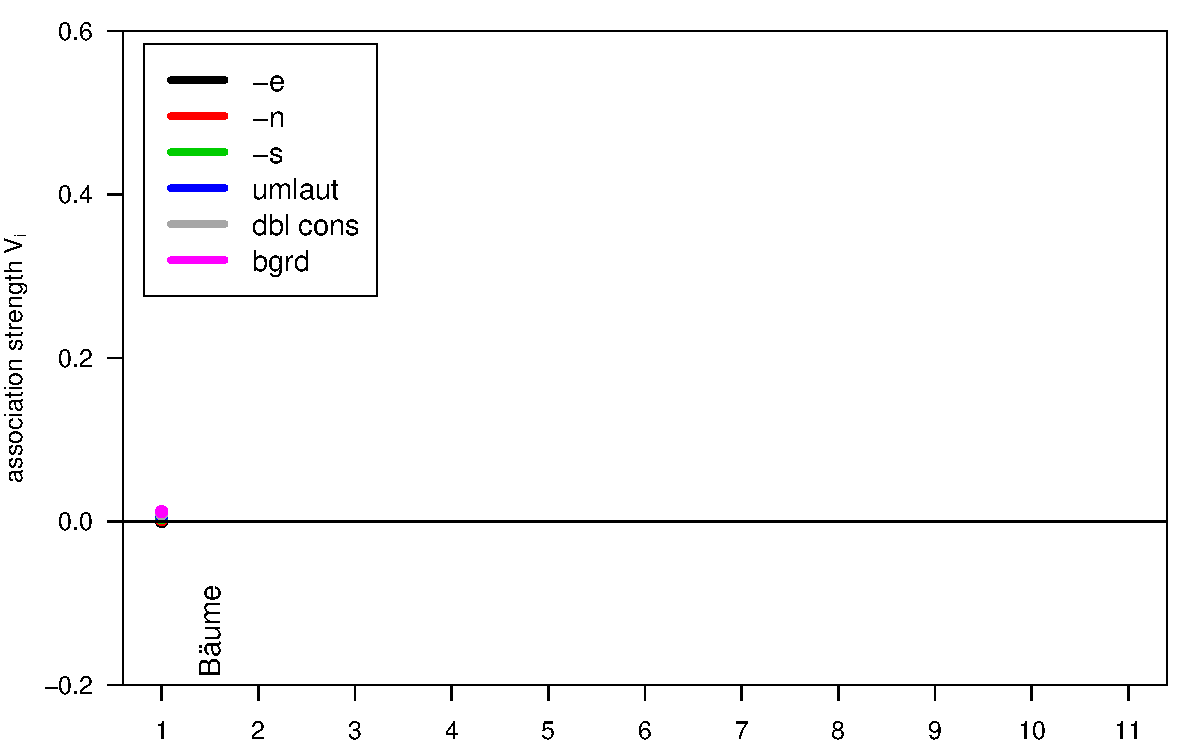
\includegraphics[width=8cm]{img/german_plural_rw_step_1}}%
  \only<beamer:2| handout:0>{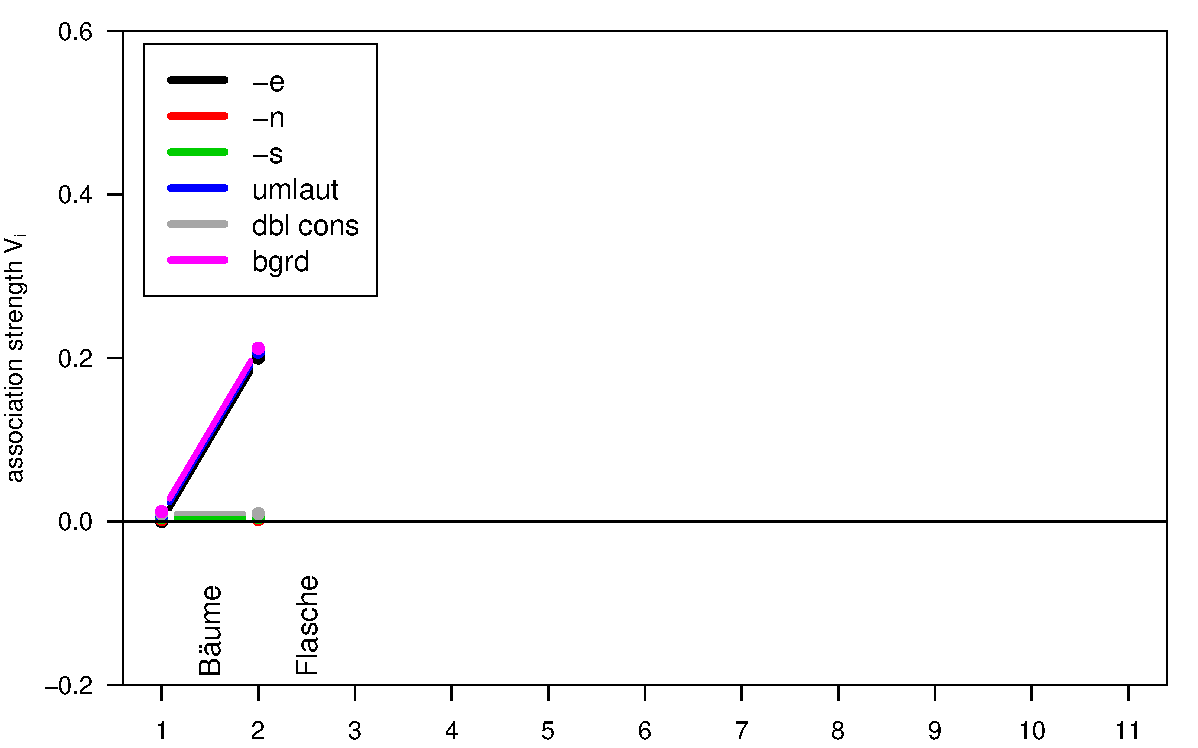
\includegraphics[width=8cm]{img/german_plural_rw_step_2}}%
  \only<beamer:3| handout:0>{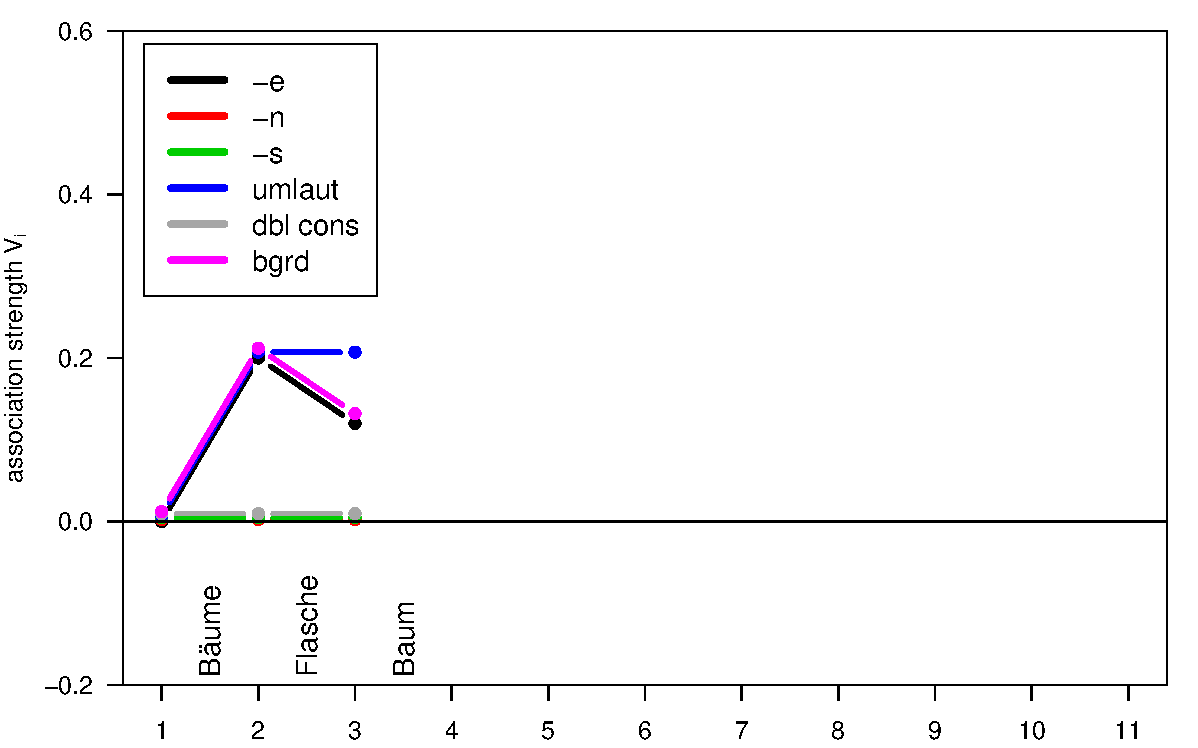
\includegraphics[width=8cm]{img/german_plural_rw_step_3}}%
  \only<beamer:4| handout:0>{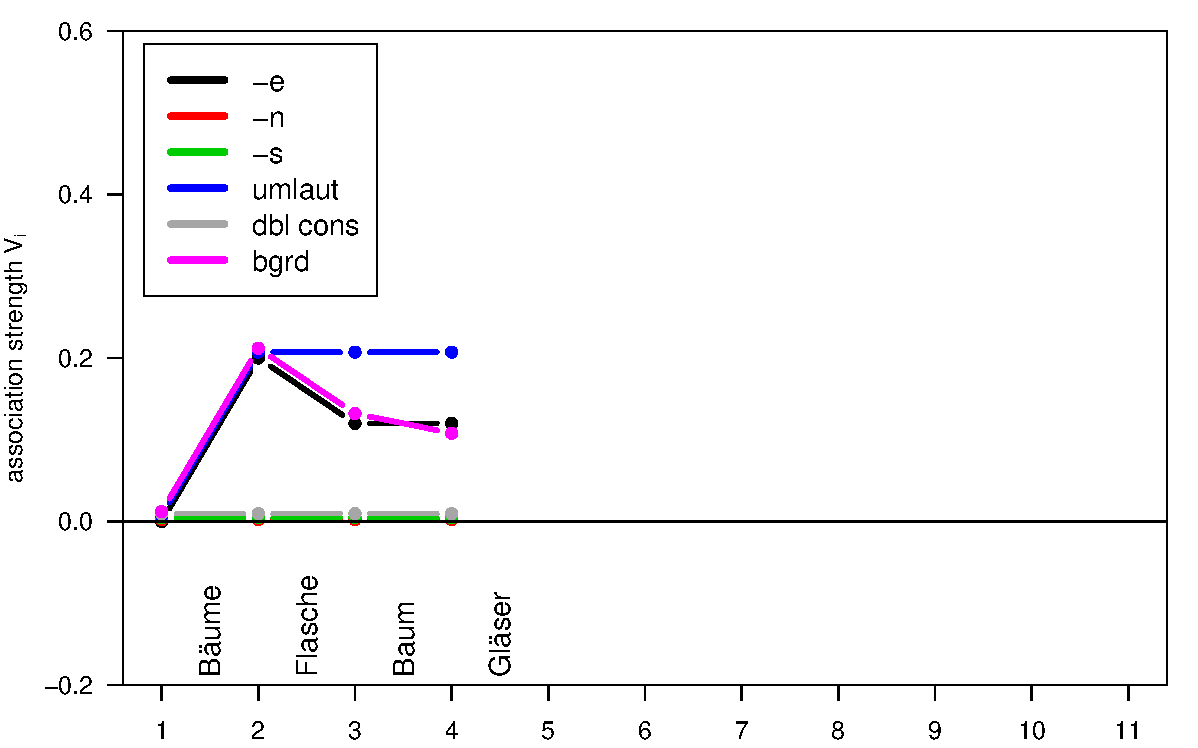
\includegraphics[width=8cm]{img/german_plural_rw_step_4}}%
  \only<beamer:5| handout:0>{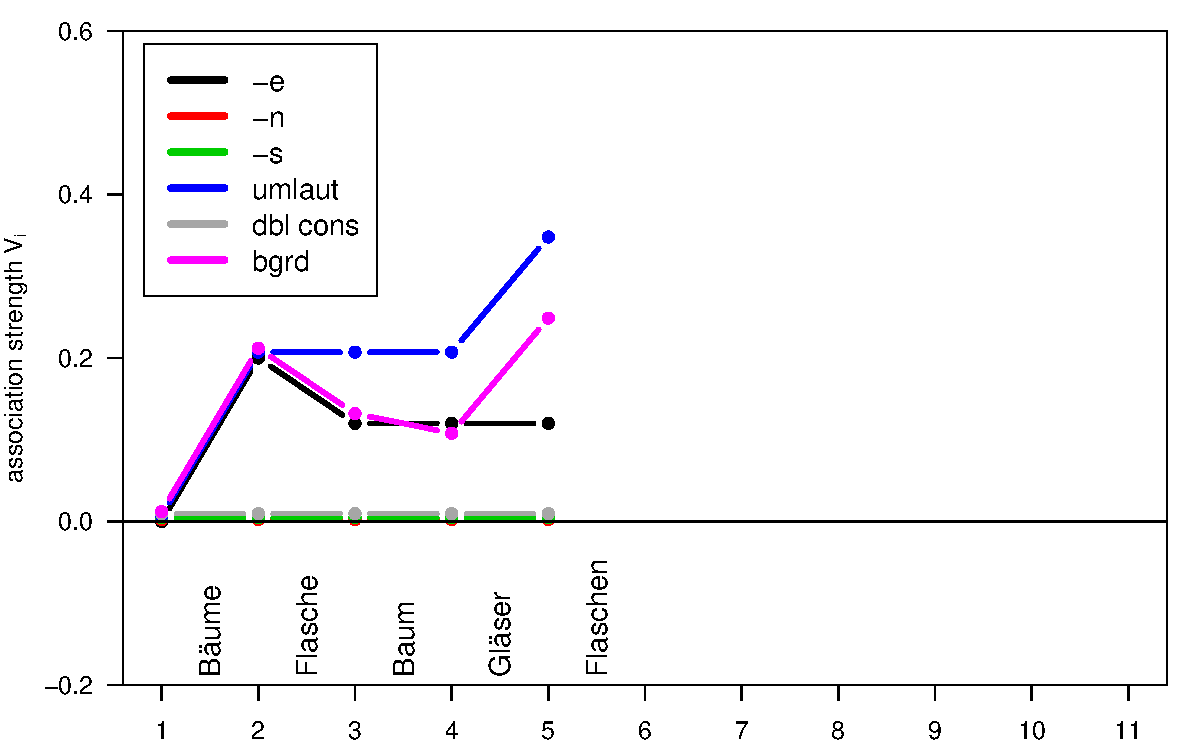
\includegraphics[width=8cm]{img/german_plural_rw_step_5}}%
  \only<beamer:6| handout:0>{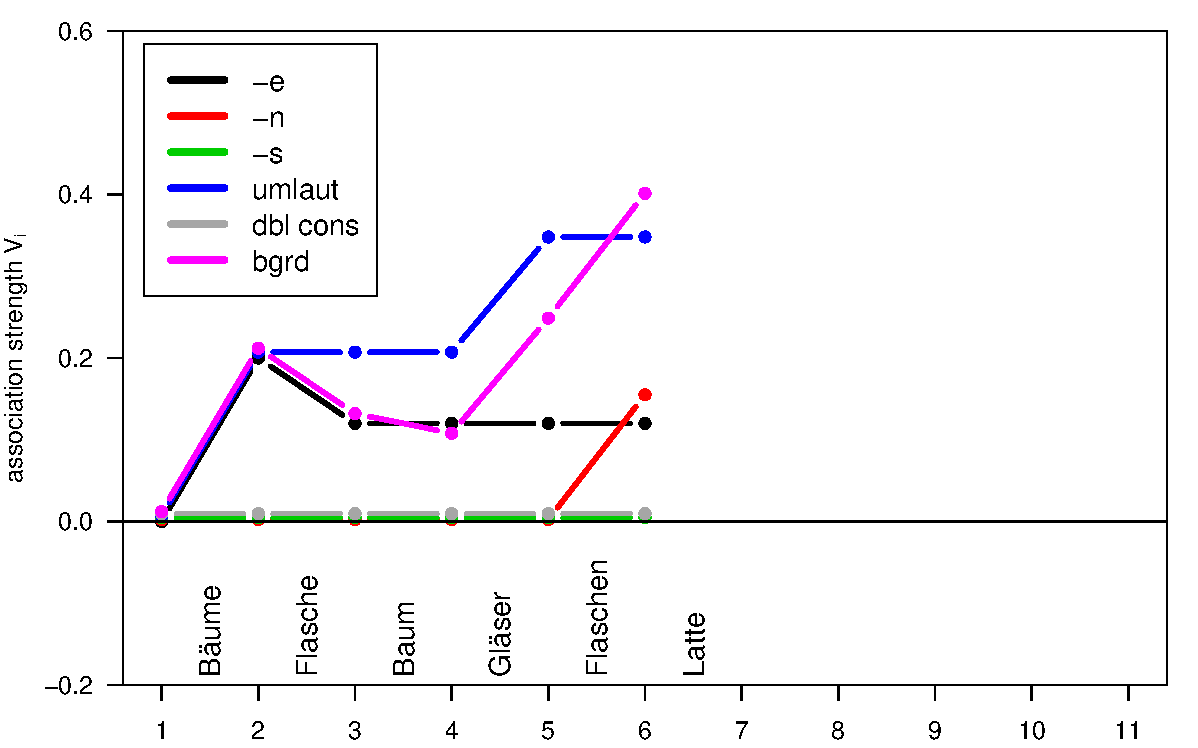
\includegraphics[width=8cm]{img/german_plural_rw_step_6}}%
  \only<beamer:7| handout:0>{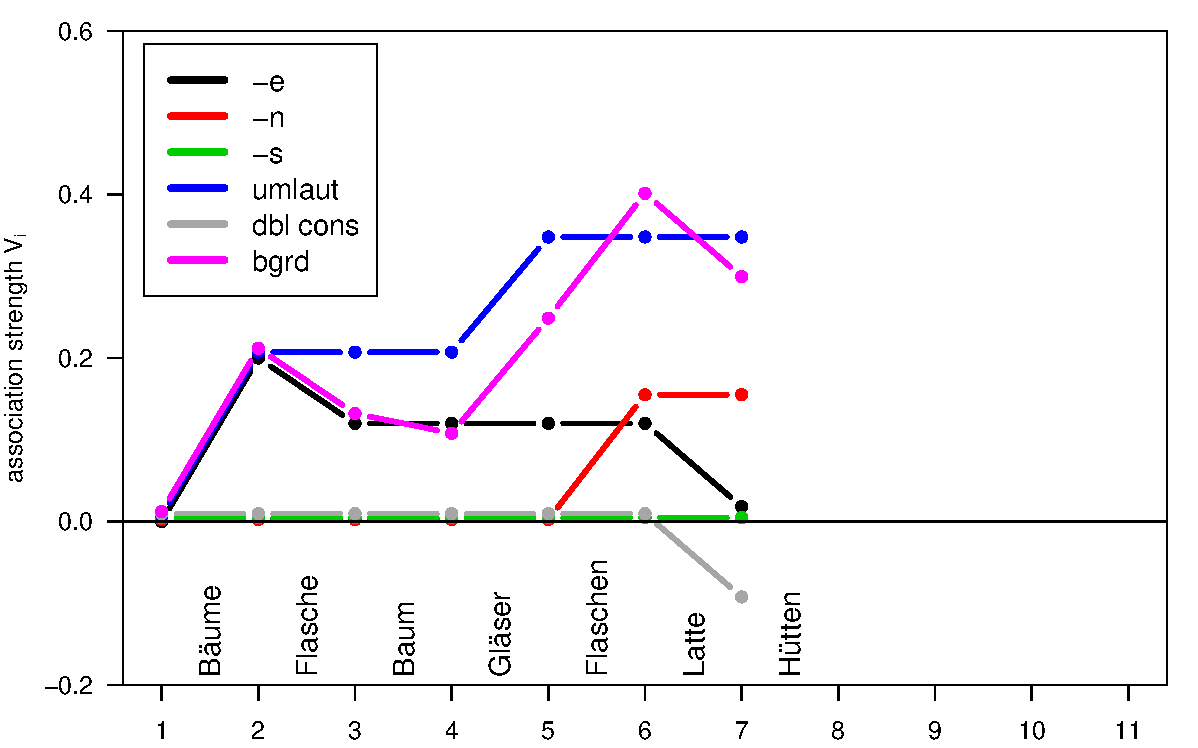
\includegraphics[width=8cm]{img/german_plural_rw_step_7}}%
  \only<beamer:8| handout:0>{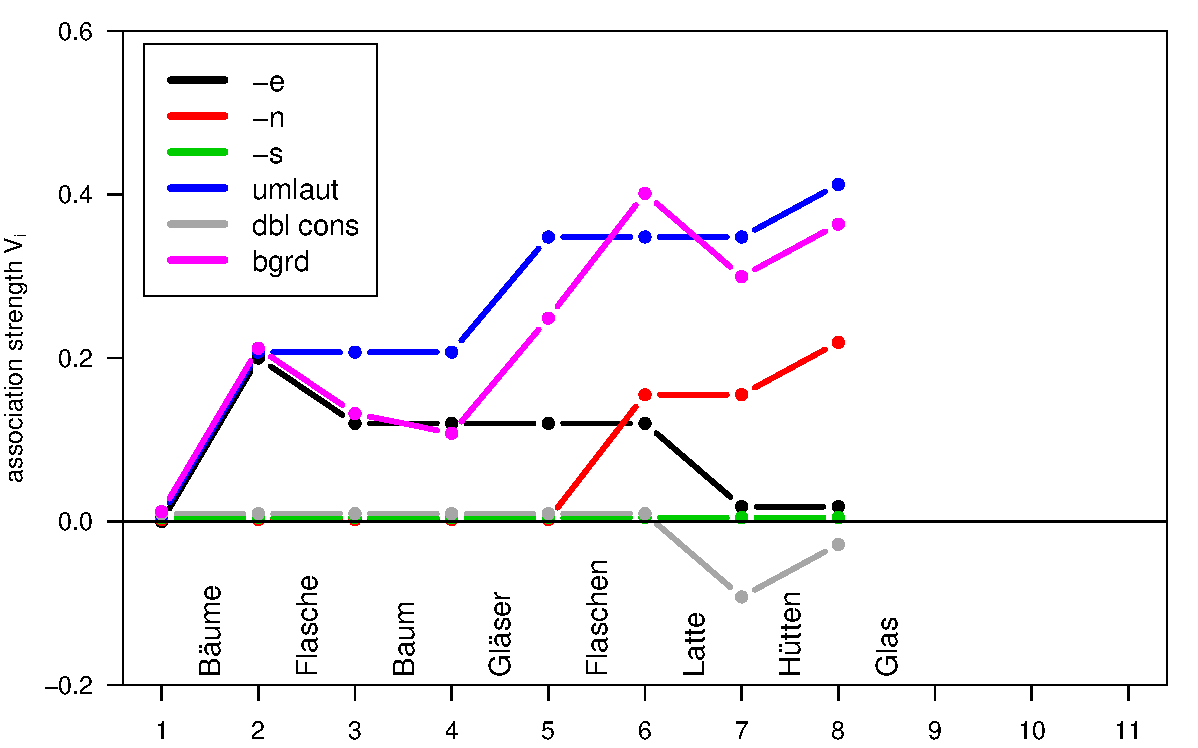
\includegraphics[width=8cm]{img/german_plural_rw_step_8}}%
  \only<beamer:9| handout:0>{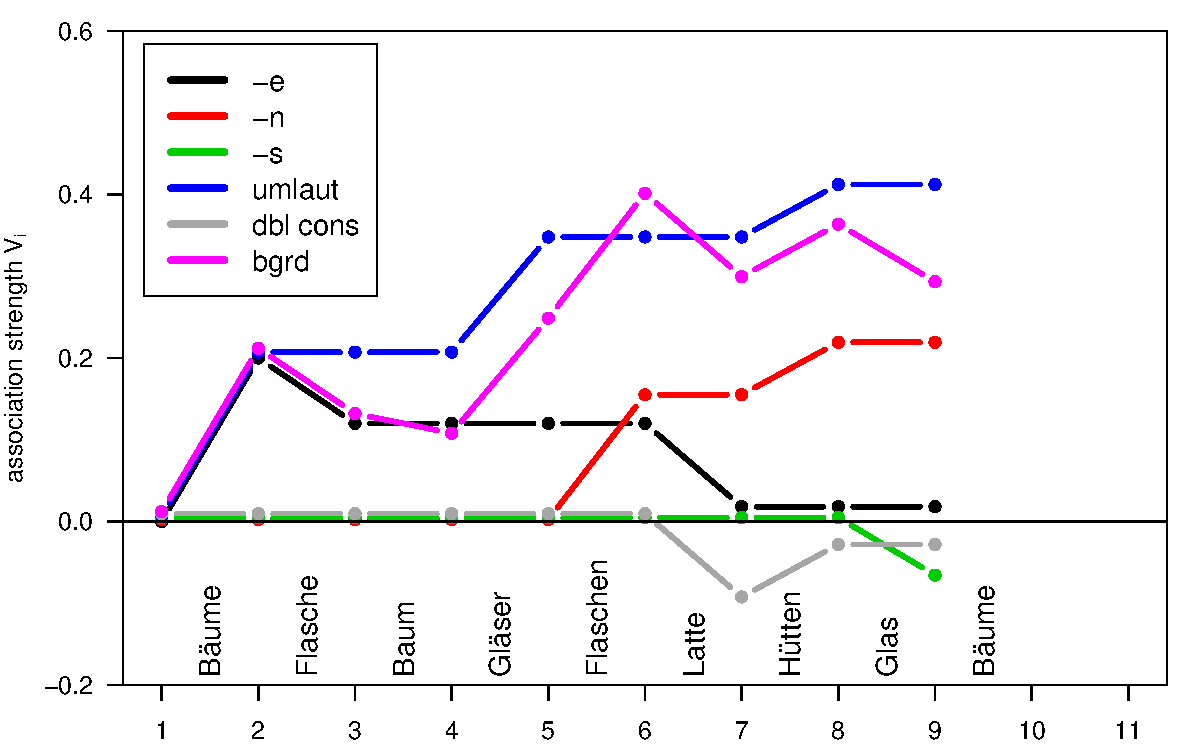
\includegraphics[width=8cm]{img/german_plural_rw_step_9}}%
  \only<beamer:10| handout:1>{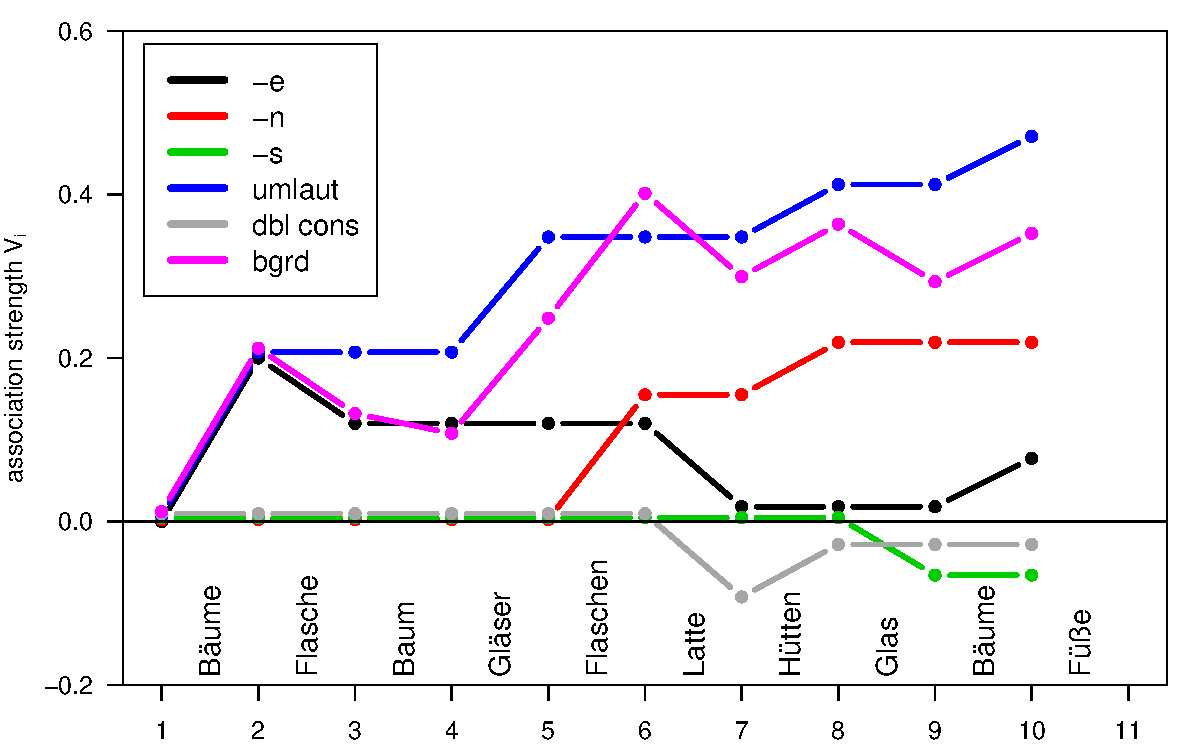
\includegraphics[width=8cm]{img/german_plural_rw_step_10}}%
  \only<beamer:11| handout:0>{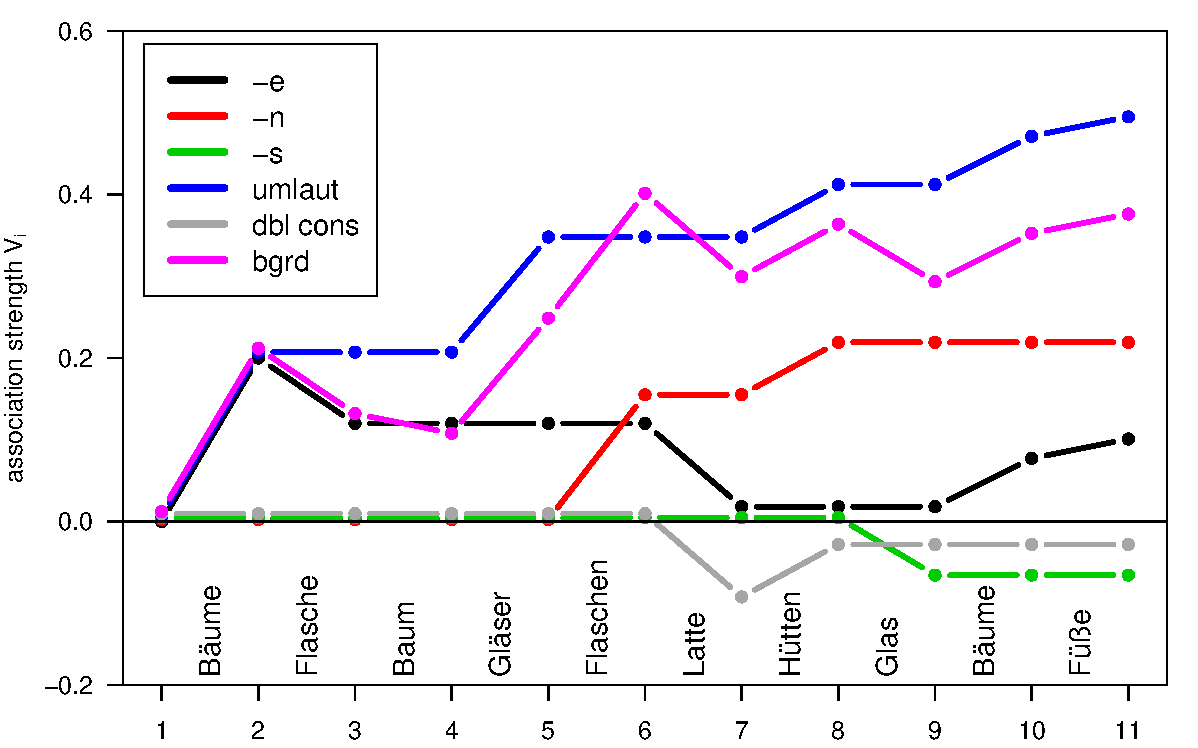
\includegraphics[width=8cm]{img/german_plural_rw_step_11}}%
\end{frame}

\begin{frame}
  \frametitle{A stochastic NDL learner}
  %% \framesubtitle{}

  \begin{itemize}
  \item<1-> A specific event sequence $(\vc[t], o\psupt)$ will only be encountered in controlled experiments
  \item<2-> For applications in corpus linguistics, it is more plausible to assume that events are randomly sampled from a population of \primary{event tokens} $(\vc[k], o\psup{k})$ for $k = 1, \ldots, m$
    \begin{itemize}
    \item[\hand] event types listed repeatedly proportional to their frequency
    \end{itemize}
  \item<3-> I.i.d.\ random variables $\vc[t] \sim \vc$ and $o\psupt\sim o$
    \begin{itemize}
    \item[\hand] distributions of $\vc$ and $o$ determined by population
    \end{itemize}
  \item<3-> NDL can now be trained for arbitrary number of time steps, even if population is small (as in our example)
    \begin{itemize}
    \item study asymptotic behaviour of learners
    \item convergence \so stable ``adult'' state of associations
    \end{itemize}
  \end{itemize}
\end{frame}

\begin{frame}[c]
  \frametitle{A stochastic NDL learner}
  \framesubtitle{Effect of the learning rate $\beta$}

  \centering\ungap[1]
  \only<beamer:1| handout:1>{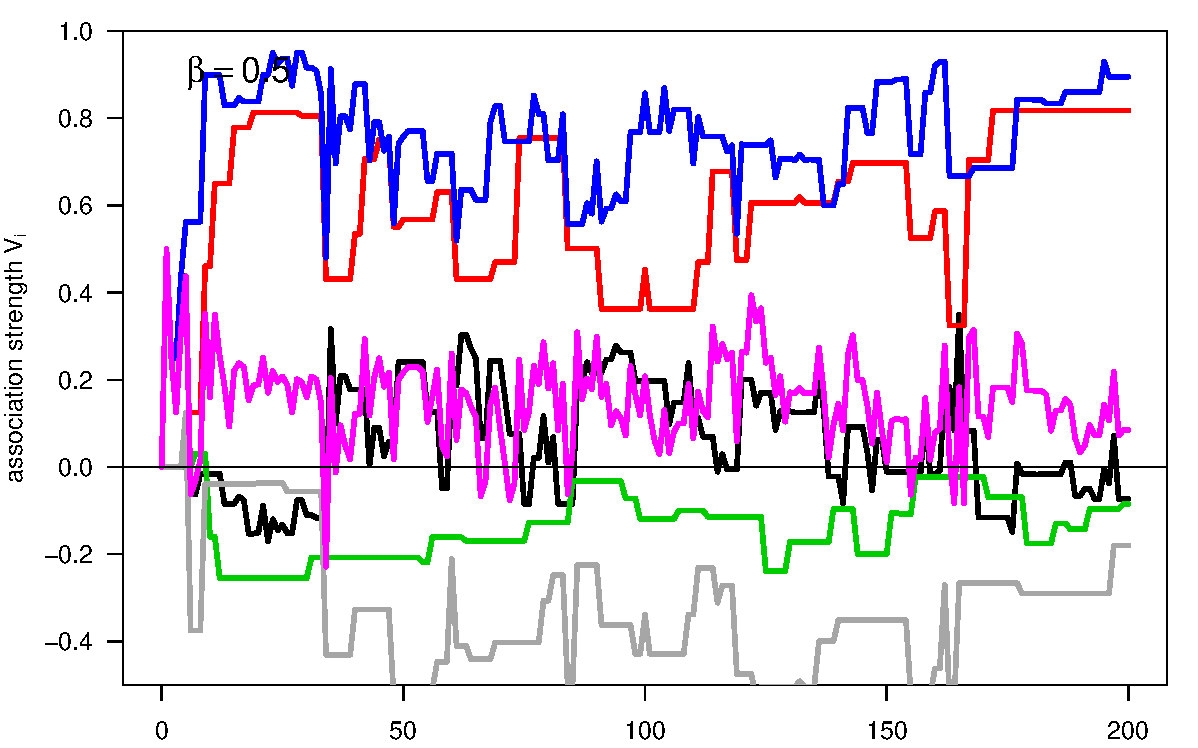
\includegraphics[width=11cm]{img/german_plural_rw_b050_n200}}%
  \only<beamer:2| handout:0>{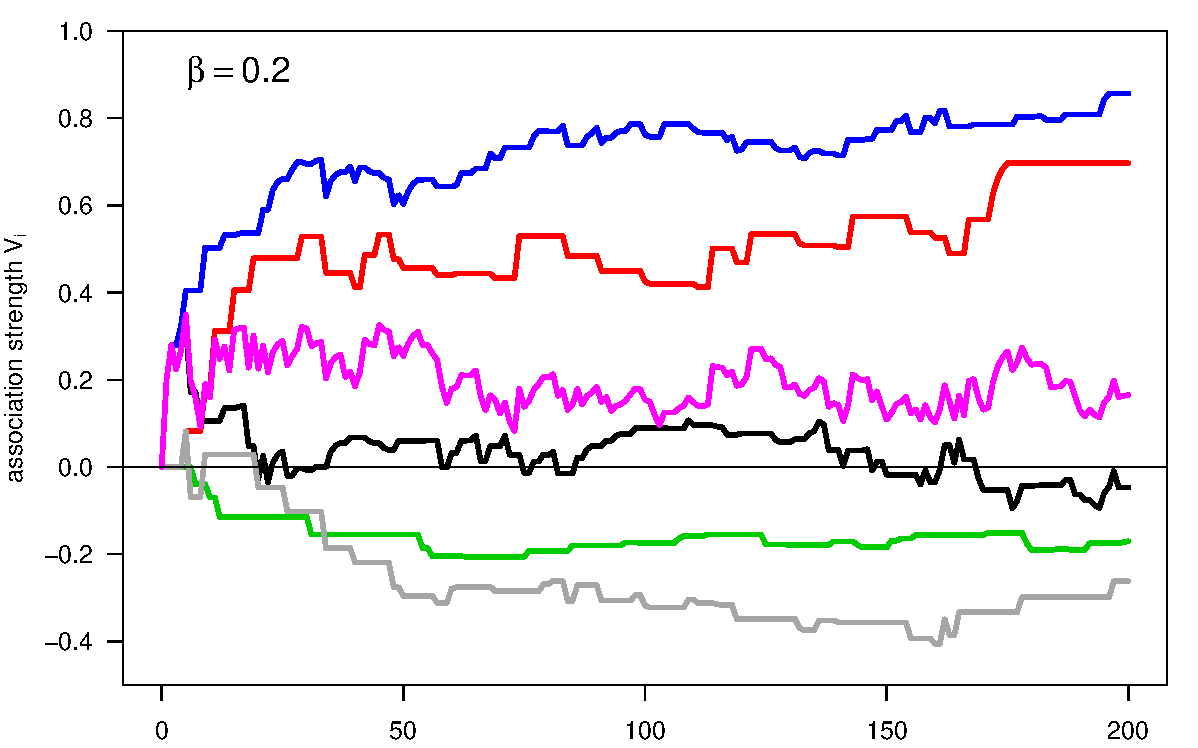
\includegraphics[width=11cm]{img/german_plural_rw_b020_n200}}%
  \only<beamer:3| handout:0>{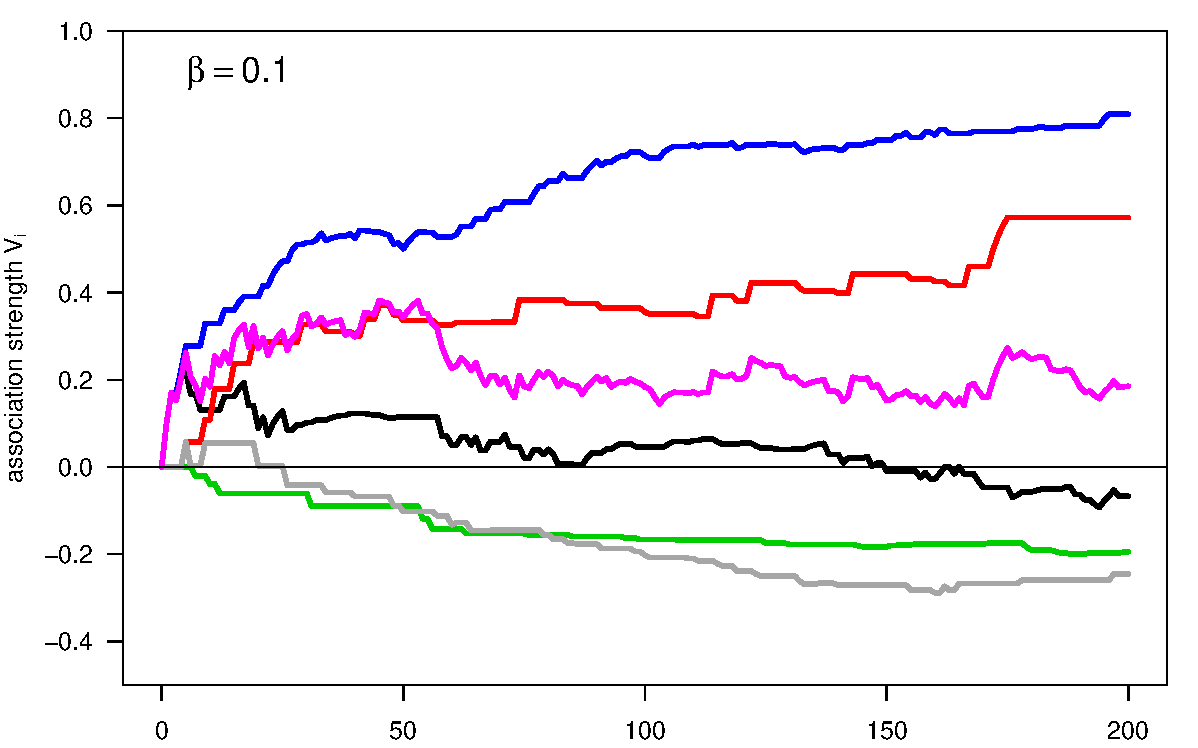
\includegraphics[width=11cm]{img/german_plural_rw_b010_n200}}%
  \only<beamer:4| handout:2>{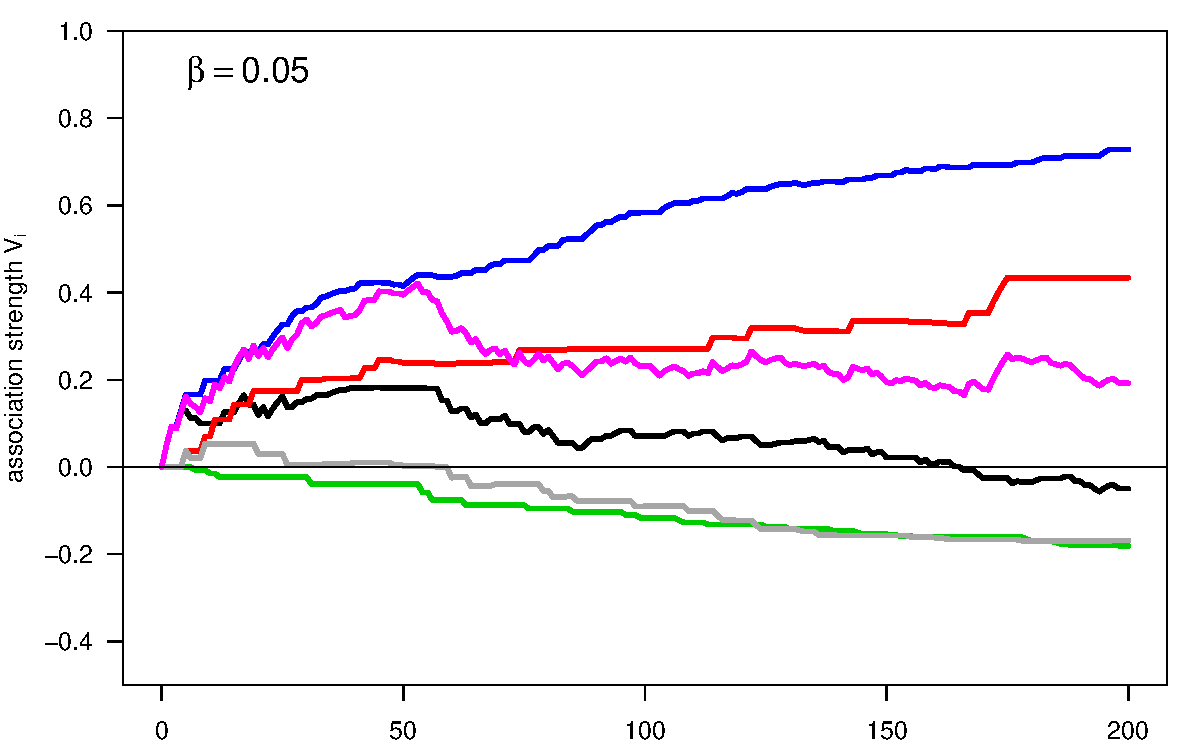
\includegraphics[width=11cm]{img/german_plural_rw_b005_n200}}%
  \only<beamer:5| handout:0>{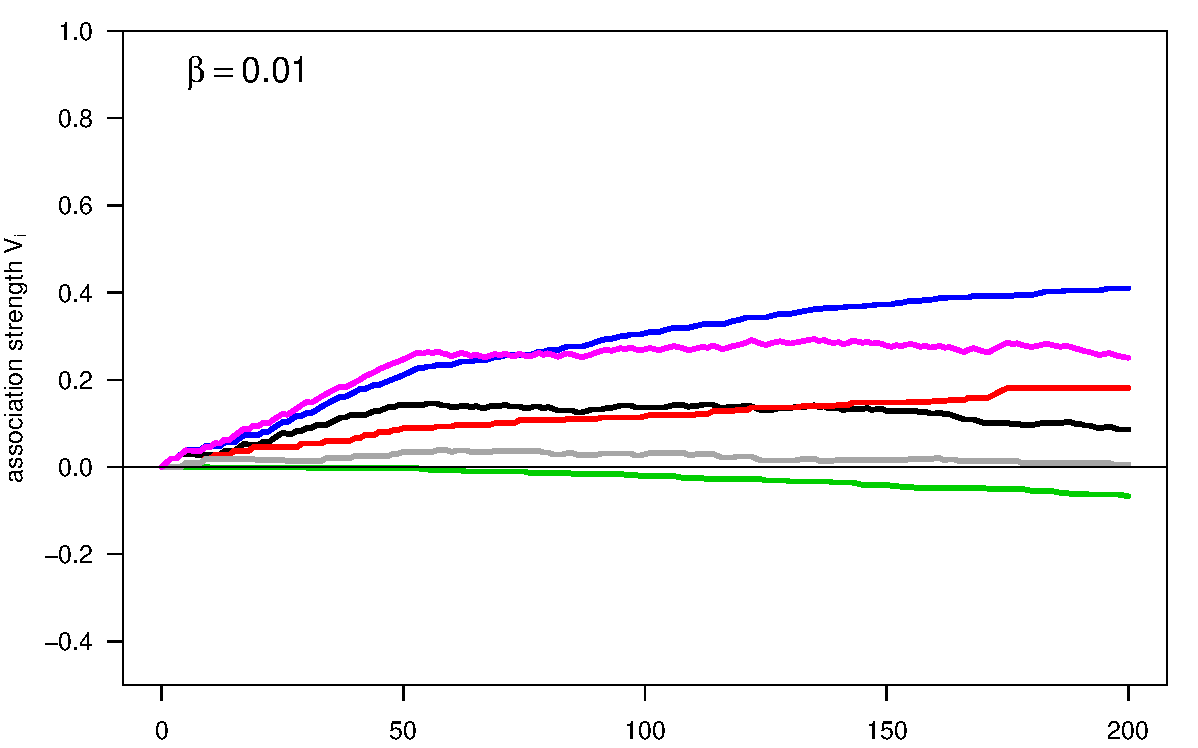
\includegraphics[width=11cm]{img/german_plural_rw_b001_n200}}%
  \only<beamer:6| handout:0>{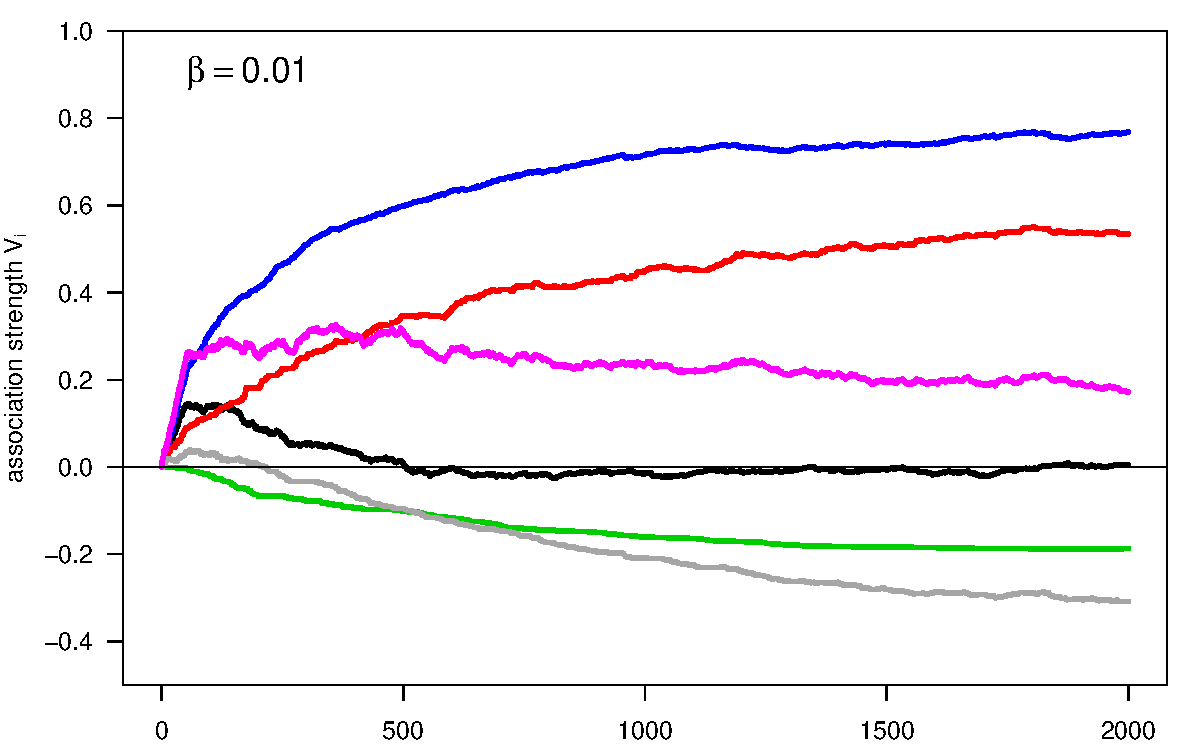
\includegraphics[width=11cm]{img/german_plural_rw_b001_n2000}}%
\end{frame}

%%%%%%%%%%%%%%%%%%%%%%%%%%%%%%%%%%%%%%%%%%%%%%%%%%%%%%%%%%%%%%%%%%%%%% 
\subsection{The Danks equilibrium}

\begin{frame}
  \frametitle{Expected activation levels}
  %% \framesubtitle{}

  \begin{itemize}
  \item Since we are interested in the general behaviour of a stochastic NDL, it makes sense to average over many individual learners to obtain \primary{expected associations} $\bigExp{V_j\psupt}$
  \end{itemize}

  \[
  \bigExp{V_{j}\psup{t+1}} = \bigExp{V_j\psupt} + \bigExp{\Delta V_j\psupt}
  \]

  \ungap[.5]
  \begin{align*}
    \bigExp{\Delta V_j\psupt} 
    &= \Expscale{ 
      c_i \beta \bigl( o - \textstyle\sum_{j=1}^n c_j V_j\psupt \bigr)
      } \qquad\qquad\qquad\qquad \\
    & \only<beamer:2| handout:0>{
      = \beta\cdot \bigExp{c_i o} - \beta\cdot \Expscale{c_i \textstyle\sum_{j=1}^n c_j V_j\psupt}
      }%
      \only<beamer:3| handout:0>{
      = \beta\cdot \bigExp{c_i o} - \beta\cdot \textstyle\sum_{j=1}^n \secondary{\bigExp{c_i c_j V_j\psupt}}
      }%
      \only<beamer:4| handout:0>{
      = \beta\cdot \secondary{\bigExp{c_i o}} - \beta\cdot \textstyle\sum_{j=1}^n \secondary{\bigExp{c_i c_j}} \bigExp{V_j\psupt}
      }% 
      \only<beamer:5| handout:1>{
      = \beta\cdot\left( \p{C_i, O} - \textstyle\sum_{j=1}^n \p{C_i, C_j} \bigExp{V_j\psupt} \right)
      }% 
  \end{align*}

  \begin{itemize}
  \item<3-> $c_i$ and $c_j$ are independent from $V_j\psupt$
  \item<4-> indicator variables: $\Exp{c_i o} = \p{C_i, O}$; $\Exp{c_i c_j} = \p{C_i, C_j}$
  \end{itemize}
\end{frame}

\begin{frame}
  \frametitle{Expected activation levels}
  %% \framesubtitle{}
  
  \ungap[1.5]
  \[
  \only<beamer:1-5| handout:0>{\Delta V_j\psupt = c_i\psupt \beta \bigl( o\psupt - \textstyle\sum_{j=1}^n c_j\psupt V_j\psupt \bigr)}%
  \only<beamer:6-| handout:1>{\bigExp{\Delta V_j\psupt} = \beta\cdot\bigl( \p{C_i, O} - \textstyle\sum_{j=1}^n \p{C_i, C_j} \bigExp{V_j\psupt} \bigr)}%
  \]
  
  \centering
  \only<beamer:1| handout:0>{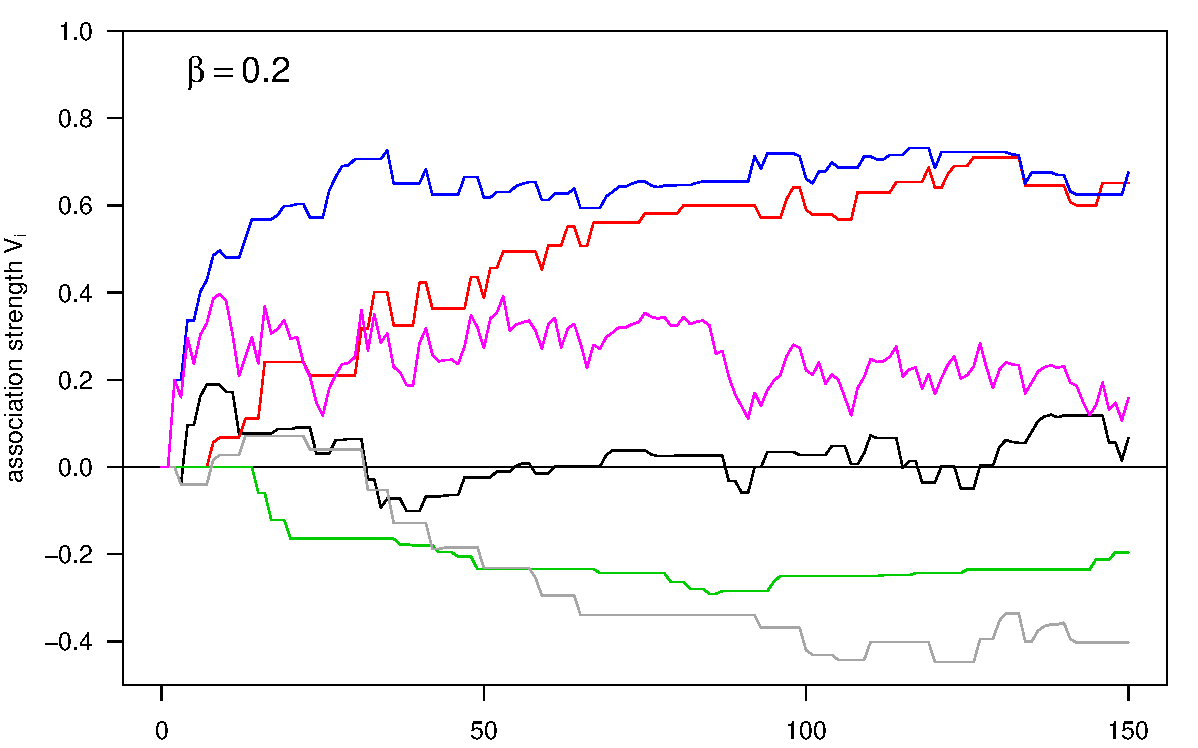
\includegraphics[width=10cm]{img/german_plural_exp_rw_step_1}}%
  \only<beamer:2| handout:0>{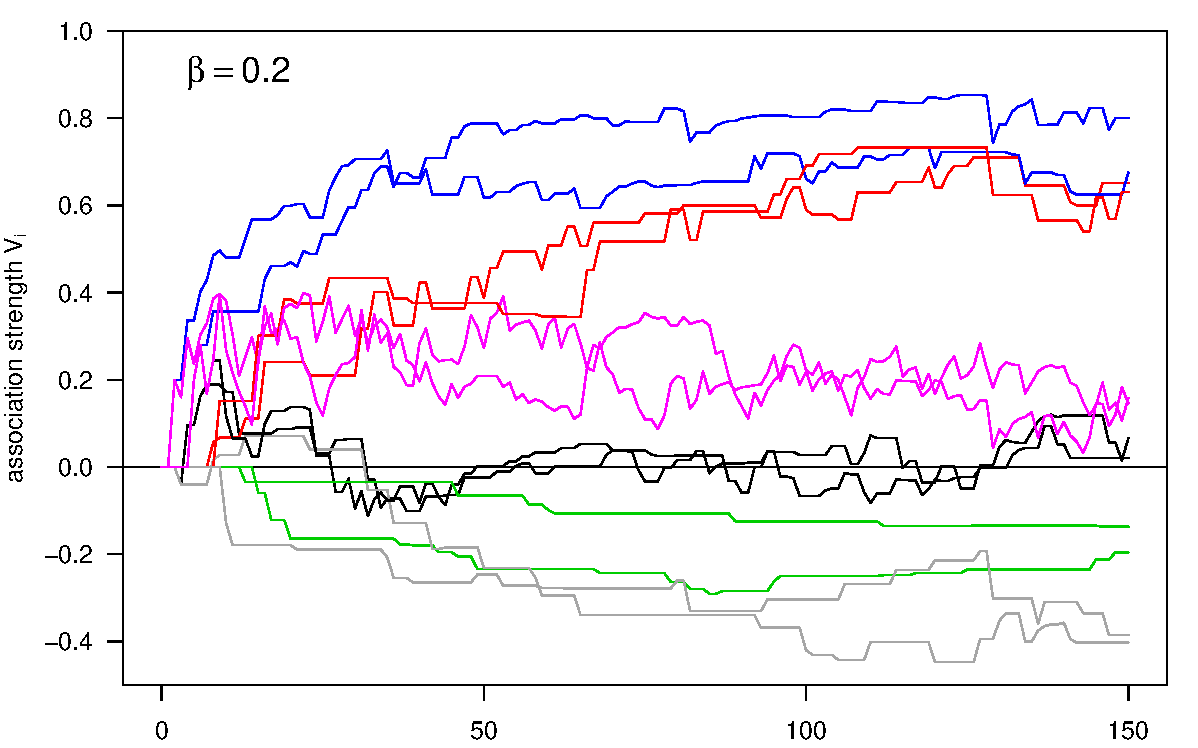
\includegraphics[width=10cm]{img/german_plural_exp_rw_step_2}}%
  \only<beamer:3| handout:0>{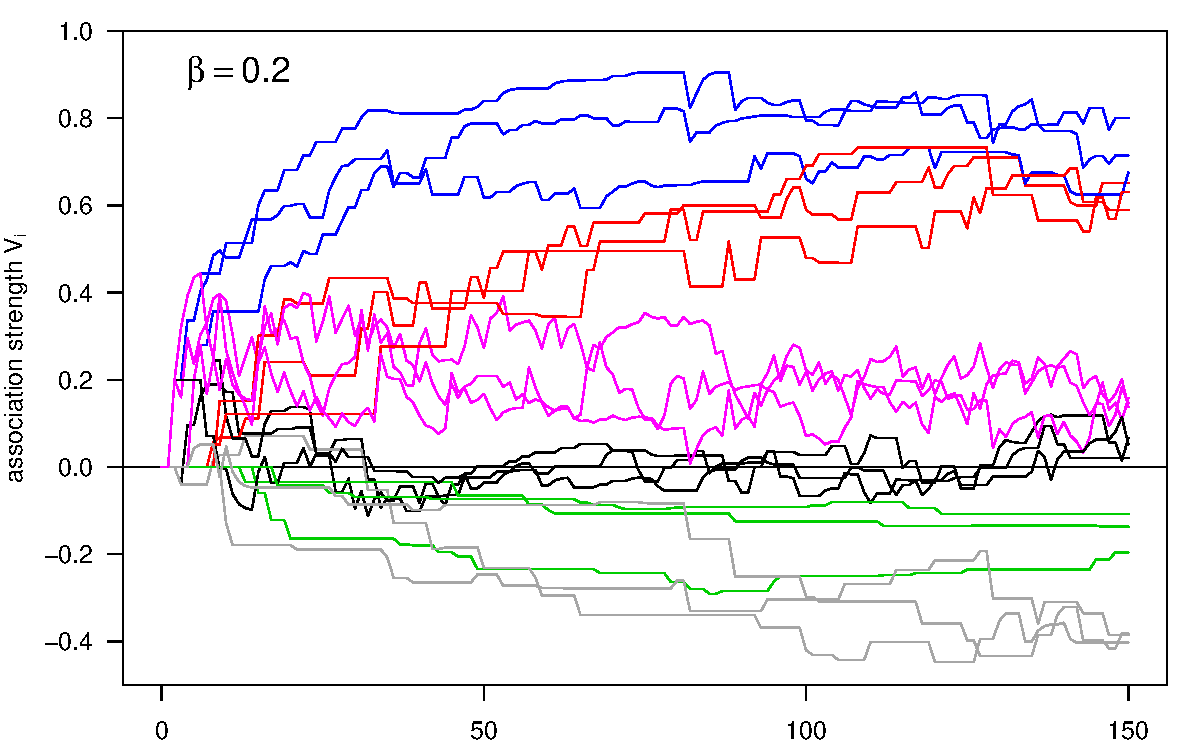
\includegraphics[width=10cm]{img/german_plural_exp_rw_step_3}}%
  \only<beamer:4| handout:0>{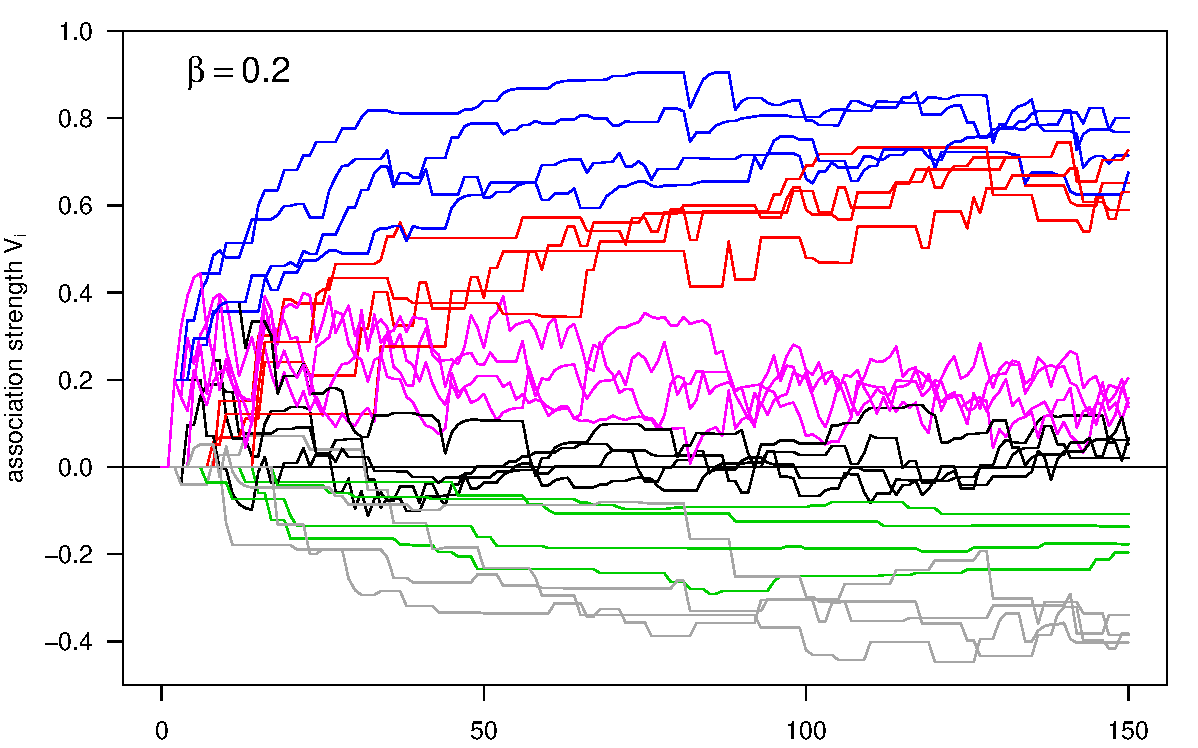
\includegraphics[width=10cm]{img/german_plural_exp_rw_step_4}}%
  \only<beamer:5| handout:0>{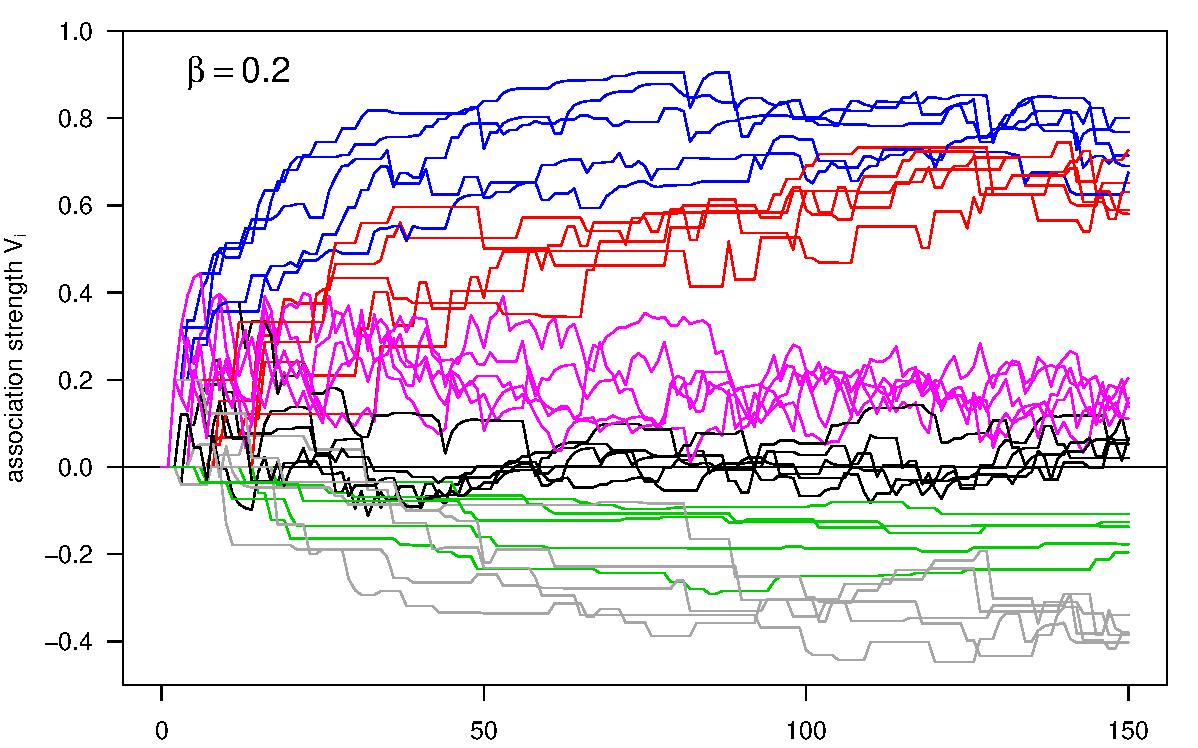
\includegraphics[width=10cm]{img/german_plural_exp_rw_step_5}}%
  \only<beamer:6| handout:1>{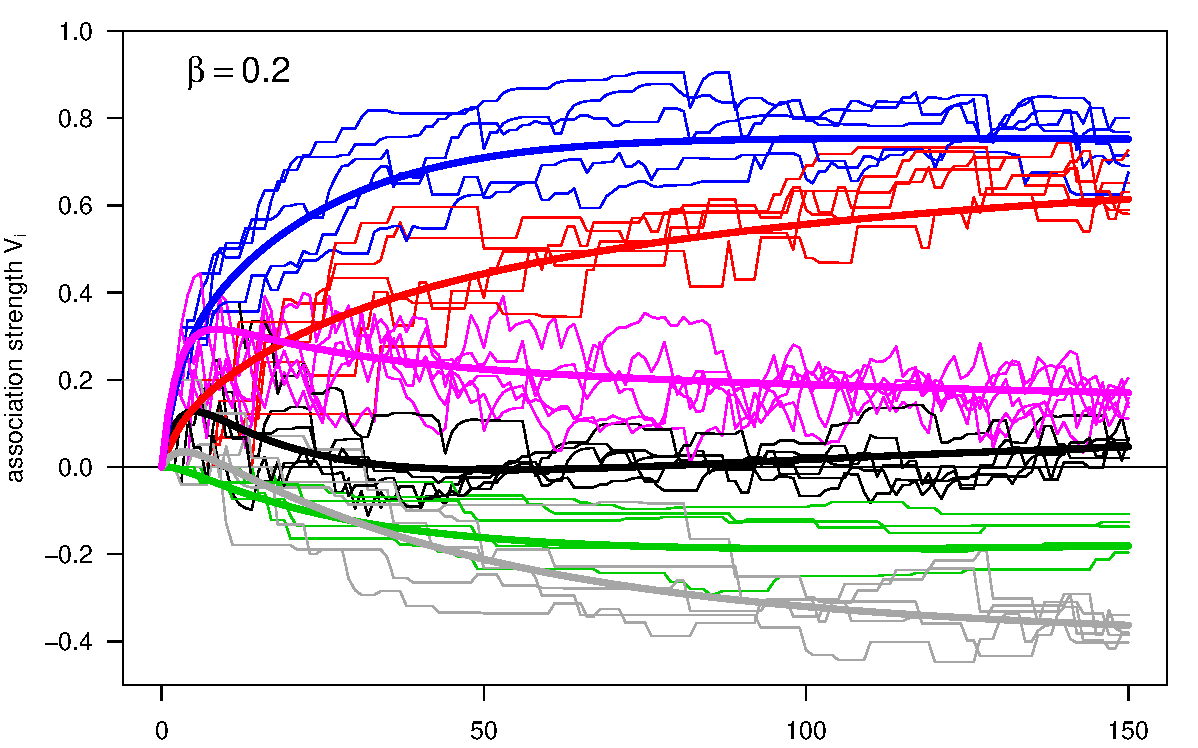
\includegraphics[width=10cm]{img/german_plural_exp_rw_final}}%
\end{frame}

\begin{frame}
  \frametitle{The Danks equilibrium}
  %% \framesubtitle{}

  \begin{itemize}
  \item If $\bigExp{V_i\psupt}$ converges, the asymptote $V_i^* = \lim_{t\to \infty} \bigExp{V_i\psupt}$ must satisfy the \primary{Danks equilibrium} conditions $\bigExp{\Delta V_i^*} = 0$, i.e.
    \[
    \p{C_i, O} - \textstyle\sum_{j=1}^n \p{C_i, C_j} V_j^* = 0 \quad \forall i
    \]
    \citep[p.~113]{Danks:03}
    \begin{itemize}
    \item[]
    \end{itemize}
  \item Now there is a clear interpretation of the Danks equilibrium as the stable average associations reached by a community of stochastic learners with input from the same population
    \begin{itemize}
    \item[\hand] allows us to compute the ``adult'' state of NDL without carrying out a simulation of the learning process
    \end{itemize}
  \end{itemize}
\end{frame}

\begin{frame}[c]
  \frametitle{The Danks equilibrium}
  %% \framesubtitle{}

  \centering
  \only<beamer:1| handout:0>{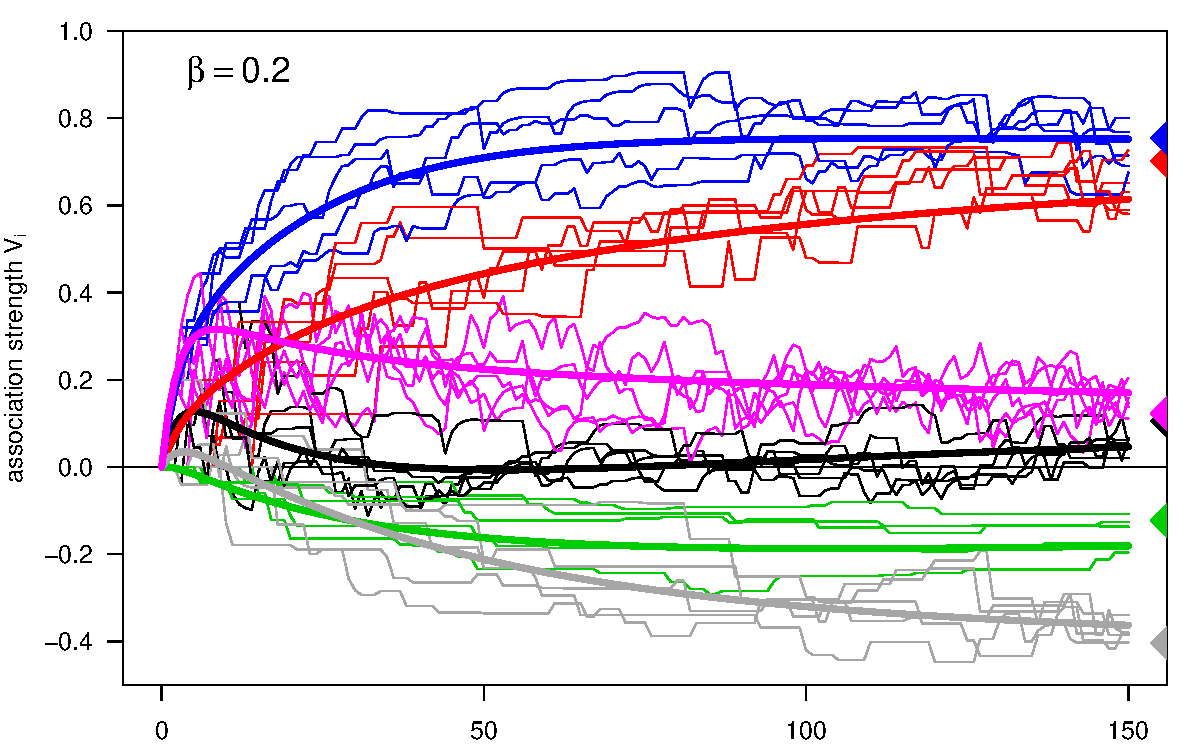
\includegraphics[width=11cm]{img/german_plural_exp_rw_danks}}%
  \only<beamer:2| handout:1>{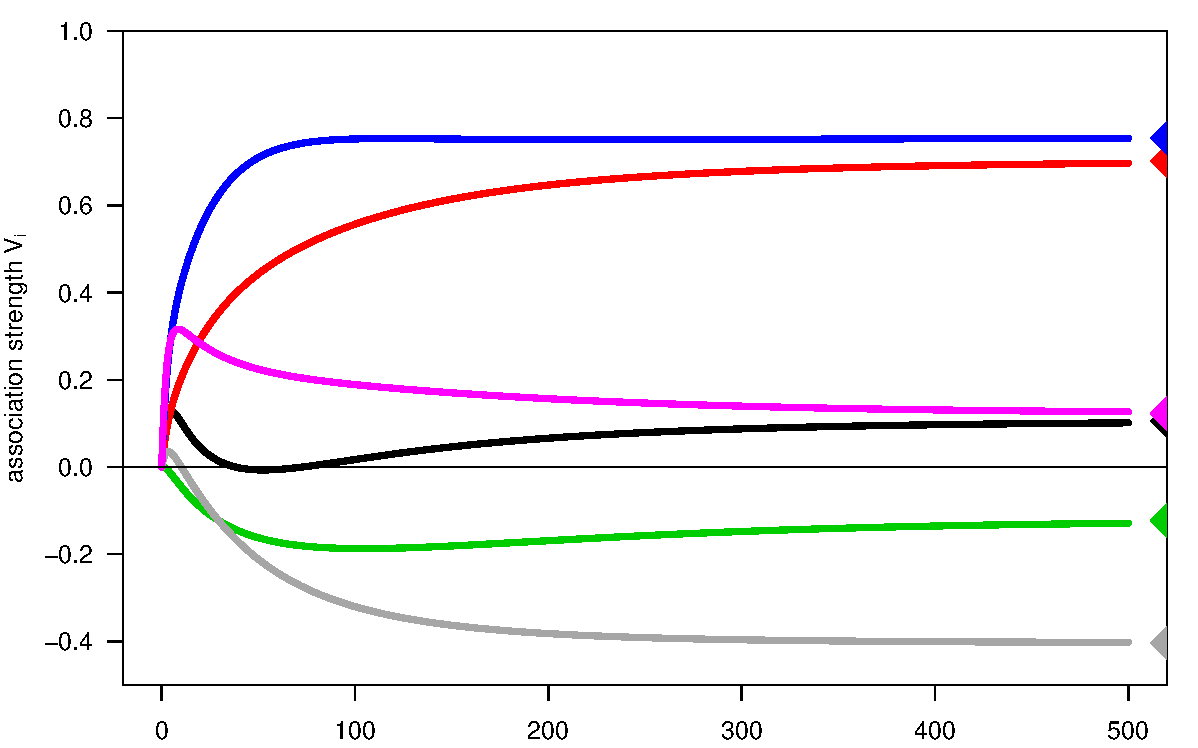
\includegraphics[width=11cm]{img/german_plural_exp_rw_danks_500}}%
\end{frame}

\begin{frame}
  \frametitle{Matrix notation}
  %% \framesubtitle{}
  
  \ungap[2]
  \begin{align*}
    \vX &=
    \begin{bmatrix}
      c_1\psup{1} & \cdots & c_n\psup{1} \\
      c_1\psup{2} & \cdots & c_n\psup{2} \\
      \vdots      &        & \vdots      \\
      c_1\psup{m} & \cdots & c_n\psup{m} 
    \end{bmatrix}
    &
    \vz &=
    \begin{bmatrix}
      o\psup{1} \\
      o\psup{2} \\
      \vdots \\
      o\psup{m}
    \end{bmatrix}
    &
    \vw &=
    \begin{bmatrix}
      V\psup{1} \\
      \vdots \\
      V\psup{n}
    \end{bmatrix}
  \end{align*}
  
  \begin{align*}
    \only<beamer:2-3| handout:0>{
    \small\begin{bmatrix} 
      f(C_1, O) \\ 
      \vdots \\
      f(C_n, O) 
    \end{bmatrix}
    &= \vX^T \vz
    &
    \visible<3->{
    \small\begin{bmatrix} 
      f(C_1, C_1) & \cdots & f(C_1, C_n) \\ 
      \vdots      &       & \vdots \\
      f(C_n, C_1) & \cdots & f(C_n, C_n)
    \end{bmatrix}
    &= \vX^T \vX
    }}%
    \only<beamer:4-| handout:1>{
    \small\begin{bmatrix} 
      \p{C_1, O} \\ 
      \vdots \\
      \p{C_n, O}
    \end{bmatrix}
    &= \tfrac{1}{m} \vX^T \vz
    &
    \small\begin{bmatrix} 
      \p{C_1, C_1} & \cdots & \p{C_1, C_n} \\ 
      \vdots      &       & \vdots \\
      \p{C_n, C_1} & \cdots & \p{C_n, C_n}
    \end{bmatrix}
    &= \tfrac{1}{m} \vX^T \vX
    }
  \end{align*}
  
  \gap[1]
  \[
  \visible<5->{\text{\primary{Danks equilibrium:}}} \quad
  \only<beamer:5| handout:0>{\tfrac{1}{m} \vX^T \vz - \tfrac{1}{m} \vX^T \vX \vw^* = \vnull}%
  \only<beamer:6-| handout:1>{\vX^T \vz = \vX^T \vX \vw^*}%
  \]
\end{frame}

\begin{frame}
  \frametitle{Matrix notation: German noun plurals}
  %% \framesubtitle{}
  
  \ungap[2]
  \begin{align*}
    \vX &=
    \footnotesize\begin{bmatrix}
      1 & 0 & 0 & 1 & 0 & 1 \\ 
      1 & 0 & 0 & 0 & 0 & 1 \\ 
      0 & 0 & 0 & 0 & 0 & 1 \\ 
      0 & 0 & 0 & 1 & 0 & 1 \\ 
      0 & 1 & 0 & 0 & 0 & 1 \\ 
      1 & 0 & 0 & 0 & 1 & 1 \\ 
      0 & 1 & 0 & 1 & 1 & 1 \\ 
      0 & 0 & 1 & 0 & 0 & 1 \\      
      1 & 0 & 0 & 1 & 0 & 1 \\ 
      1 & 0 & 0 & 1 & 0 & 1
    \end{bmatrix}
    &
    \vz &=
    \footnotesize\begin{bmatrix}
      1  \\
      0  \\
      0  \\
      1  \\
      1  \\
      0  \\
      1  \\
      0  \\
      1  \\
      1 
    \end{bmatrix}
    &
    \vw &=
    \begin{bmatrix}
      V\psup{1} \\
      \vdots \\
      V\psup{n}
    \end{bmatrix}
  \end{align*}
  
  \begin{align*}
    \only<beamer:1-3| handout:0>{
    \visible<2->{
    \small\begin{bmatrix} 
      3 \\ 
      2 \\
      0 \\
      5 \\
      1 \\
      6
    \end{bmatrix}
    &= \vX^T \vz}
    &
    \visible<3->{
    \small\begin{bmatrix} 
      5 & 0 & 0 & 3 & 1 &  5 \\ 
      0 & 2 & 0 & 1 & 1 &  2 \\ 
      0 & 0 & 1 & 0 & 0 &  1 \\ 
      3 & 1 & 0 & 5 & 1 &  5 \\ 
      1 & 1 & 0 & 1 & 2 &  2 \\ 
      5 & 2 & 1 & 5 & 2 & 10 
    \end{bmatrix}
    &= \vX^T \vX}
    }%
    \only<beamer:4-| handout:1>{
    \small\begin{bmatrix} 
      .3 \\ 
      .2 \\
      .0 \\
      .5 \\
      .1 \\
      .6
    \end{bmatrix}
    &= \tfrac{1}{m} \vX^T \vz
    &
    \small\begin{bmatrix} 
      .5 & .0 & .0 & .3 & .1 &  .5 \\ 
      .0 & .2 & .0 & .1 & .1 &  .2 \\ 
      .0 & .0 & .1 & .0 & .0 &  .1 \\ 
      .3 & .1 & .0 & .5 & .1 &  .5 \\ 
      .1 & .1 & .0 & .1 & .2 &  .2 \\ 
      .5 & .2 & .1 & .5 & .2 &  1 
    \end{bmatrix}
    &= \tfrac{1}{m} \vX^T \vX
    }
  \end{align*}
\end{frame}

%%%%%%%%%%%%%%%%%%%%%%%%%%%%%%%%%%%%%%%%%%%%%%%%%%%%%%%%%%%%%%%%%%%%%%
\subsection{NDL vs.\ the Perceptron vs.\  least-squares regression}

\tikzset{input/.style={basic,circle}}
\tikzset{weights/.style={basic,rectangle}}
\tikzset{functions/.style={basic,circle,fill=faugold!10}}
\tikzset{basic/.style={draw,fill=faublue!10,text width=1em,text badly centered}}
%% \tikzset{flow/.style={draw,-{>[scale=1.2]}}} % nicer, but only works with PGF 3.0
\tikzset{flow/.style={draw,->}} % nicer, but only works with PGF 3.0

\begin{frame}
  \frametitle{The single-layer perceptron (SLP)}
  %% \framesubtitle{}

  \begin{columns}[c]
    \begin{column}{6cm}
      SLP \citep{Rosenblatt:58} is the most basic feed-forward \primary{neural network}
      \begin{itemize}
      \item<1-> numeric inputs $x_1, \ldots, x_n$
      \item<1-> output activation $h(y)$ based on weighted sum of inputs
        \[
        y = \textstyle\sum_{j=1}^n w_j x_j
        \]
      \item<2-> $h$ = Heaviside step function in traditional SLP
      \item<3-> even simpler model: $h(y) = y$
      \item<4-> cost wrt.\ target output $z$:
        \[
        E(\vw, \vx, z) = \left( z - \textstyle\sum_{j=1}^n w_j x_j \right)^2
        \]
      \end{itemize}
    \end{column}
    \begin{column}{5cm}
      \begin{tikzpicture}
        \node[functions] (center) {};
        \node[below=0.5em of center,font=\scriptsize,text width=3.4em] {activation function $h$};
        \draw (0em,0.75em) -- (0em,-0.75em);
        \draw (0.75em,0em) -- (-0.75em,0em);
        \only<beamer:1-2| handout:0>{
          \draw[very thick, color=primary] (0.7em,0.5em) -- (0,0.5em) -- (0,-0.5em) -- (-0.7em,-0.5em);
        }
%%        \draw[very thick, color=primary] (0.7em,0.5em) .. controls (-0.2em,0.5em) and (0.2em,-0.5em) .. (-0.7em,-0.5em);
        \only<beamer:3-| handout:1>{
          \draw[very thick, color=primary] (0.6em,0.6em) -- (-0.6em,-0.6em);
        }
        \node[right of=center] (right) {};
        \path[flow] (center) -- (right);
        \node[functions,left=1.5em of center] (left) {$\sum$};
        \path[flow] (left) -- (center);
        \node[weights,above left=0.5em and 2em of left] (2) {$w_2$} -- (2) node[input,left=1em of 2] (l2) {$x_2$};
        \path[flow] (l2) -- (2);
        \path[flow] (2) -- (left);
        \node[below of=2] (dots) {$\vdots$} -- (dots) node[below of=l2] (ldots) {$\vdots$};
        \node[weights,below of=dots] (n) {$w_n$} -- (n) node[input,left=1em of n] (ln) {$x_n$};
        \path[flow] (ln) -- (n);
        \path[flow] (n) -- (left);
        \node[weights,above of=2] (1) {$w_1$} -- (1) node[input,left=1em of 1] (l1) {$x_1$};
        \path[flow] (l1) -- (1);
        \path[flow] (1) -- (left);
        \node[below=1.5em of ln.center,font=\scriptsize] {inputs};
        \node[below=1.5em of n.center,font=\scriptsize] {weights};
      \end{tikzpicture}
    \end{column}
  \end{columns}  
\end{frame}

\begin{frame}
  \frametitle{SLP training: the delta rule}
  %% \framesubtitle{}
  \begin{itemize}
  \item SLP weights are learned by \primary{gradient descent} training:\\
    for a single training item $(\vx, z)$ and learning rate $\delta > 0$
    \begin{align*}
      \Delta w_i &= -\delta \frac{\partial E(\vw, \vx, z)}{\partial w_i} \\
      \only<beamer:1-2| handout:0>{\visible<2->{&= -\delta \frac{\partial}{\partial w_i} \left( z - \sum_{j=1}^n w_j x_j \right)^2 \\}}
      \only<beamer:3-4| handout:0>{&= -2\delta \left( z - \sum_{j=1}^n w_j x_j \right) (-x_i) \\}
      \only<beamer:5-| handout:1>{&= 2\delta x_i \left( z - \sum_{j=1}^n x_ j w_j \right) \\}
      \visible<4->{&= \secondary{\beta c_i \bigl( o - \textstyle\sum_{j=1}^n c_j V_j \bigr)}}
    \end{align*}
  \item<6-> Perfect \primary{correspondence to W-H rule} with
    \[
    V_i = w_i \qquad c_i = x_i \qquad o = z \qquad \beta = 2\delta
    \]
  \end{itemize}
\end{frame}

\begin{frame}
  \frametitle{Batch training}
  %% \framesubtitle{}

  \begin{itemize}
  \item Neural networks often use \primary{batch training}, where all training data are considered at once instead of one item at a time
  \item Similar to stochastic NDL, batch training computes the expected weights $\bigExp{\vw\psupt}$ for a SLP with stochastic input
  \item<2-> The corresponding batch training cost is
    \begin{align*}
    E(\vw) &= \frac{1}{m} \sum_{k=1}^m E(\vw, \vx[k], z\psup{k}) \\
    \visible<3->{ &= \frac{1}{m} \sum_{k=1}^m \left( z\psup{k} - \textstyle\sum_{j=1}^n w_j x_j\psup{k} \right)^2 }
    \end{align*}
  \item<3-> Minimization of $E(\vw)$ = linear \primary{least-squares regression}
  \end{itemize}
\end{frame}

\begin{frame}
  \frametitle{Linear least-squares regression}
  %% \framesubtitle{}
  
  \begin{itemize}
  \item Matrix formulation of the linear least-squares problem:
    \begin{align*}
      E(\vw) &= \frac{1}{m} \sum_{k=1}^m \left( z\psup{k} - \textstyle\sum_{j=1}^n w_j x_j\psup{k} \right)^2 \\
      \visible<2->{ &= \frac{1}{m} \bigl( \vz - \vX \vw \bigr)^T \bigl( \vz - \vX \vw \bigr) }
    \end{align*}
  \item<3-> Minimum of $E(\vw)$, the $L_2$ solution, must satisfy $\nabla E(\vw^*) = \vnull$, which leads to the \primary{normal equations}
    \[
    \vX^T \vz = \vX^T \vX \vw^*
    \]
  \item<4-> Normal equations = Danks equilibrium conditions
  \item<5-> Regression theory shows that batch training / stochastic NLP converges to the unique$^{\primary{*}}$ solution of the $L_2$ problem
  \end{itemize}
\end{frame}

\begin{frame}[c]
  \frametitle{What have we learned?}
  %% \framesubtitle{}

  \begin{center}\Large
    \setlength{\fboxrule}{2pt}
    \fcolorbox{secondary}{faugold!10!white}{
      \begin{tabular}{c c c c c}
        stochastic &=& batch &=& $L_2$ regression \\[1ex]
        NDL &=& SLP
      \end{tabular}
    }
  \end{center}  

  \begin{itemize}
  \item<2->[\hand] These equivalences also hold for the general R-W equations with arbitrary values of $\alpha_i$, $\beta_1$, $\beta_2$ and $\lambda$
    \begin{itemize}
    \item salience-adjusted weights: $w_i = V_i / \sqrt{\alpha_i}$  
    \item scaled outcome indicators: $z = \lambda o$
    \item scaled cue indicators:
      \[
        x_i = 
        \begin{cases}
          \sqrt{\alpha_i} & \text{if } c_i = 1 \wedge o = 1 \\
          \sqrt{\alpha_i} \sqrt{\frac{\beta_2}{\beta_1}} & \text{if } c_i = 1 \wedge o = 0 \\
          0 & \text{otherwise}
        \end{cases}
      \]
    \end{itemize}
  \end{itemize}

\end{frame}

\begin{frame}
  \frametitle{Effects of R-W parameters}
  %% \framesubtitle{}

  
  \begin{description}
  \item<1->[$\beta > 0$:] learning rate \so convergence of individual learners
  \item<2->[$\lambda \neq 1$:]\gap[.5] linear scaling of associations / activation (obvious)
  \item<3->[$\alpha_i\neq 1$:]\gap[.5] salience of cue $C_i$ determines how fast associations are learned, but does not affect the final stable associations (same $L_2$ regression problem)
  \item<4->[$\beta_1 \neq \beta_2$:]\gap[.5] different positive/negative learning rates \emph{do} affect the stable associations; closely related to prevalence of positive and negative events in the population
  \end{description}
\end{frame}



%%%%%%%%%%%%%%%%%%%%%%%%%%%%%%%%%%%%%%%%%%%%%%%%%%%%%%%%%%%%%%%%%%%%%%
%% 3 NLP
\section{Natural language processing}

%%%%%%%%%%%%%%%%%%%%%%%%%%%%%%%%%%%%%%%%%%%%%%%%%%%%%%%%%%%%%%%%%%%%%%
\subsection{Machine learning in NLP}

\begin{frame}
  \frametitle{The last 50 years of computational linguistics}

  \begin{center}
    \begin{tabular}{lp{4cm}p{5cm}}
      1970s & Rule-based approaches & Toy worlds, expert systems \\
            & & \\
      \onslide<2->
      1980s & Linguistic theories & \\
            & Formal language theory & \\
      \onslide<3->
      1990s & & Large corpora\\
            & Probabilistic models & \\
      \onslide<4->
      2000s & & Supervised classification \\
            & Machine learning & \\
      \onslide<5->
      2010s & & \\
            & Deep learning (RNN) & \\
      2020s & & End-to-end learning
    \end{tabular}
  \end{center}
\end{frame}

\begin{frame}
  \frametitle{NLP as supervised classification}
  \newcommand{\out}{\color<2->{fourth!20!white}}%
  \newcommand{\bdry}{\primary{$\,$\rule{1pt}{1em}\raisebox{1ex}{$^?\!\!$}}}%
  
  \h{Part-of-speech tagging}

  \begin{center}\large
    \begin{tabular}{cccccccc}
      & \code{JJ} & & & & & \\
      \code{\out RB} & \code{\out VVP} & \code{\out VVP} & \code{VVZ} & & \code{\out VVZ} & \\
      \code{DT} & \code{\out NN} & \code{NN} & \code{\out NNS} & \code{CD} & \code{NNS} & \code{SENT}\\
      \textcite{This} & \textcite{light} & \textcite{brew} & \textcite{costs} & \textcite{ten} & \textcite{bucks} & \textcite{.} 
    \end{tabular}
  \end{center}

  \gap[1]
  \onslide<3->
  \h{Tokenization}

  \begin{center}\large
    \textcite{The 14\bdry F model is approx\bdry . 15\bdry cm long\bdry .}
  \end{center}
\end{frame}

\begin{frame}
  \frametitle{NLP as supervised classification}
  \newcommand{\OP}{\primary{[}}%
  \newcommand{\CL}{\primary{]}}%
  
  \h{Syntactic attachment disambiguation}

  \begin{center}
    \textcite{\large I saw the girl and the boy with glasses.}\\
    \normalsize\gap[.5]\onslide<2->
    I saw \OP{}the girl and the boy\CL{} \OP{}with glasses\CL{}\\
    I saw \OP{}\OP{}the girl and the boy\CL{} with glasses\CL{}\\
    I saw \OP{}the girl\CL{} and \OP{}the boy with glasses\CL{}
  \end{center}

  \gap[1]
  \onslide<3->
  \h{Dependency parsing}
  \begin{center}
    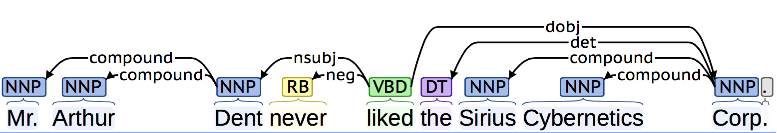
\includegraphics[width=10cm]{img/corenlp_parse2}%
  \end{center}
\end{frame}

\begin{frame}
  \frametitle{NLP as supervised classification}

  \h{Named entity recognition}
  \begin{center}\ungap[1]
    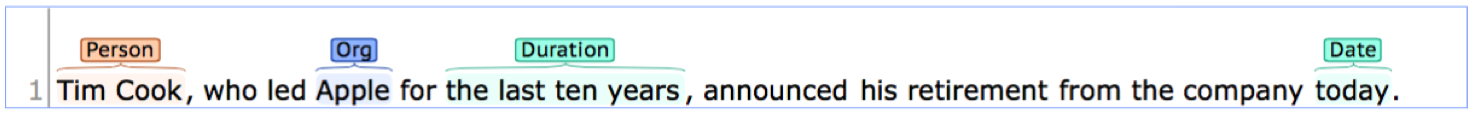
\includegraphics[width=11cm]{img/corenlp_ner}%
  \end{center}

  \gap[1]
  \onslide<2->
  \h{Semantic role labelling\\
    Word sense disambiguation\\
    Sentiment analysis\\
    Author profiling\\
    Recognizing textual entailment\\
    Automatic grading\\
    \ldots}
\end{frame}

%%%%%%%%%%%%%%%%%%%%%%%%%%%%%%%%%%%%%%%%%%%%%%%%%%%%%%%%%%%%%%%%%%%%%%
\subsection{MaxEnt and logistic regression}

\begin{frame}
  \frametitle{The maximum entropy approach (MaxEnt)}

  \begin{itemize}
  \item A popular machine learning algorithm in NLP is based on the maximum entropy principle \citep{Berger:DellaPietra:96}
  \item Estimate conditional distribution $p(y|x)$ with maximal entropy
    \[
      H(p) = -\sum_{x,y} \tilde{p}(x) p(y|x) \log p(y|x)
    \]
    so that expectations of features $f_i(x, y)$ match training data
    \[
      \Exp[p]{f_i(x, y)} = \sum_{x,y} \tilde{p}(x, y) f_i(x, y)
    \]
  \item<2->[\hand] These features represent associations between outcomes ($y$) and cues (different properties of $x$)
  \end{itemize}
\end{frame}

\begin{frame}
  \frametitle{The maximum entropy approach (MaxEnt)}

  \begin{itemize}
  \item Leads to a log-linear probability distribution
    \[
      p(y|x) \sim e^{\sum_i \lambda_i f_i(x, y)}
    \]
    whose parameters $\lambda_i$ are optimized to maximize the log-likelihood
    of the training data
  \item[]
  \item For binary $y$, this is equivalent to \primary{logistic regression}
    \begin{itemize}
    \item remember \citet{Bresnan:etc:07}?
    \end{itemize}
  \end{itemize}
\end{frame}

\begin{frame}
  \frametitle{Logistic regression and NDL}
  %% \framesubtitle{}

  \begin{columns}[T]
    \begin{column}{6cm}
      Logistic regression is the standard tool for predicting a categorical response from binary features 
      \begin{itemize}
      \item<1-> can be expressed as SLP with probabilistic interpretation
      \item<2-> uses logistic activation function
        \[
        h(y) = \frac{1}{1 + e^{-y}}
        \]
      \item<3-> and Bernoulli cost
        \[
        E(\vw, \vx, z) = \begin{cases}
          -\log h(y) & \text{if } z = 1 \\
          -\log (1 - h(y)) & \text{if } z = 0
        \end{cases}
        \]
      \end{itemize}
    \end{column}
    \begin{column}{5cm}
      \begin{tikzpicture}
        \node[functions] (center) {};
        \node[below=0.5em of center,font=\scriptsize,text width=3.4em] {activation function $h$};
        \draw (0em,0.75em) -- (0em,-0.75em);
        \draw (0.75em,0em) -- (-0.75em,0em);
        \only<beamer:1| handout:0>{
          \draw[very thick, color=primary] (0.6em,0.6em) -- (-0.6em,-0.6em);
        }
        \only<beamer:2-| handout:1>{
          \draw[very thick, color=primary] (0.7em,0.5em) .. controls (-0.2em,0.5em) and (0.2em,-0.5em) .. (-0.7em,-0.5em);
        }
        \node[right of=center] (right) {};
        \path[flow] (center) -- (right);
        \node[functions,left=1.5em of center] (left) {$\sum$};
        \path[flow] (left) -- (center);
        \node[weights,above left=0.5em and 2em of left] (2) {$w_2$} -- (2) node[input,left=1em of 2] (l2) {$x_2$};
        \path[flow] (l2) -- (2);
        \path[flow] (2) -- (left);
        \node[below of=2] (dots) {$\vdots$} -- (dots) node[below of=l2] (ldots) {$\vdots$};
        \node[weights,below of=dots] (n) {$w_n$} -- (n) node[input,left=1em of n] (ln) {$x_n$};
        \path[flow] (ln) -- (n);
        \path[flow] (n) -- (left);
        \node[weights,above of=2] (1) {$w_1$} -- (1) node[input,left=1em of 1] (l1) {$x_1$};
        \path[flow] (l1) -- (1);
        \path[flow] (1) -- (left);
        \node[below=1.5em of ln.center,font=\scriptsize] {inputs};
        \node[below=1.5em of n.center,font=\scriptsize] {weights};
      \end{tikzpicture}
    \end{column}
  \end{columns}  
\end{frame}

\begin{frame}
  \frametitle{Logistic regression and NDL}
  %% \framesubtitle{}

  \begin{itemize}
  \item Gradient descent training leads to delta rule that corresponds to a modified version of the R-W equations
    \[
    \Delta V_i =
    \begin{cases}
      0 & \text{if } c_i = 0\\
      \beta \left( 1 - h \bigl( \sum_{j=1}^n c_j V_j \bigr) \right) & \text{if } c_i = 1 \wedge o = 1 \\
      \beta \left( 0 - h \bigl( \sum_{j=1}^n c_j V_j \bigr) \right) & \text{if } c_i = 1 \wedge o = 0
    \end{cases}
    \]
  \item<2-> Same as original R-W, except that activation level is now transformed into probability $h(y)$
  \item<2-> But no easy way to analyze stochastic learning process\\
    (batch training $\neq$ expected value of single-item training)
  \item<2-> Less robust for highly predictable outcomes \so $\vw$ diverges
  \end{itemize}
\end{frame}


%%%%%%%%%%%%%%%%%%%%%%%%%%%%%%%%%%%%%%%%%%%%%%%%%%%%%%%%%%%%%%%%%%%%%%
\subsection{Conclusion}

\begin{frame}
  \frametitle{Summary \& some open questions}
  %% \framesubtitle{}
  \begin{center}
    \setlength{\fboxrule}{1pt}
    \fcolorbox{secondary}{faugold!10!white}{
      \begin{tabular}{c c c c c}
        stochastic &=& batch &=& $L_2$ regression \\[1ex]
        NDL &=& linear SLP \\[1ex]
        MaxEnt &=& sigmoid SLP &=& logistic regression
      \end{tabular}
    }
  \end{center}

  \gap[1]
  \begin{itemize}
  \item How many training steps are needed for a stochastic NDL learner to
    converge to the Danks equilibrium?
  \item What is the relation between NDL and regularized regression?
  \item How does logistic regression behave as incremental learner?
  \item Which sequences / patterns in the input data lead to significantly
    different behaviour from a stochastic learner?
  \end{itemize}

\end{frame}

\begin{frame}
  \frametitle{Acknowledgements}
  %% \framesubtitle{}

  \ungap[1]
  \begin{columns}[T]
    \begin{column}{55mm}
      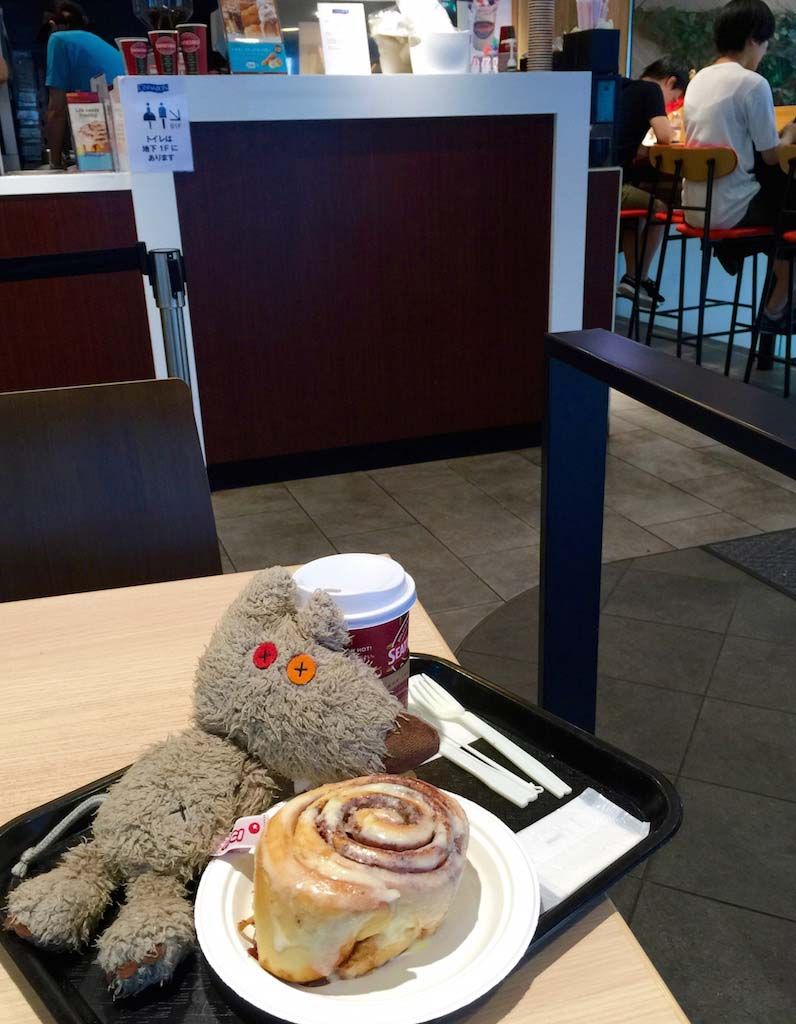
\includegraphics[width=52mm]{img/ratti_cinnamon_rolls}
      
      \scriptsize
      Follow me on Twitter: \secondary{@RattiTheRat}
    \end{column}
    \begin{column}{50mm}
      The mathematical analysis was fuelled by large amounts of coffee and cinnamon rolls at Cinnabon, Harajuku, Tokyo

      \vspace{8em}
      Based on joint research with Antti Arppe (U Alberta).
      Read \citet{Evert:Arppe:15} for the full story.
    \end{column}

  \end{columns}
\end{frame}



%%%%%%%%%%%%%%%%%%%%%%%%%%%%%%%%%%%%%%%%%%%%%%%%%%%%%%%%%%%%%%%%%%%%%%
%% References (if any)

\frame[allowframebreaks]{
  \frametitle{References}
  \bibliographystyle{natbib-stefan}
  \begin{scriptsize}
    \bibliography{references}
  \end{scriptsize}
}

\end{document}
